% 独自のコマンド

% ■ アブストラクト
%  \begin{jabstract} 〜 \end{jabstract}  :日本語のアブストラクト
%  \begin{eabstract} 〜 \end{eabstract}  :英語のアブストラクト

% ■ 謝辞
%  \begin{acknowledgment} 〜 \end{acknowledgment}

% ■ 文献リスト
%  \begin{bib}[100] 〜 \end{bib}


\newif\ifjapanese

\japanesetrue  % 論文全体を日本語で書く(英語で書くならコメントアウト)

\ifjapanese
  \documentclass[a4j,twoside,openright,11pt]{jreport} % 両面印刷の場合。余白を綴じ側に作って右起こし。
  % \usepackage[backend=bibtex]{biblatex}
  %\documentclass[a4j,11pt]{jreport}                  % 片面印刷の場合。
  \renewcommand{\bibname}{参考文献}
  \newcommand{\acknowledgmentname}{謝辞}
\else
  \documentclass[a4paper,11pt]{report}
  \newcommand{\acknowledgmentname}{Acknowledgment}
\fi
\usepackage{thesis}
\usepackage{ascmac}
\usepackage[dvipdfmx]{graphicx}
\usepackage{multirow}
\usepackage{url}
\usepackage{amsmath}
\usepackage{lscape}
%\bibliographystyle{jplain}
\bibliographystyle{junsrt}

\bindermode  % バインダー用余白設定

% 日本語情報(必要なら)
\jclass  {卒業論文}                             % 論文種別
\jtitle    {脈波を使った時系列UX評価手法に関する研究}    % タイトル。改行する場合は\\を入れる
\juniv    {慶應義塾大学}                  % 大学名
\jfaculty  {環境情報学部}               % 学部、学科
\jauthor  {佐々木 雄司}                       % 著者
\jhyear  {3}                                   % 平成○年度
\jsyear  {2021}                                 % 西暦○年度
\jkeyword  {UX, 脈波, UI, ユーザテスト, ユーザビリティ, 人間中心設計}     % 論文のキーワード
\jproject{全世界インタフェースデザイン (増井研究会)} %プロジェクト名
\jdate{2022年1月}

% 英語情報(必要なら)
\eclass  {Graduation Thesis}                            % 論文種別
\etitle    {Studies on the UX Evaluation Method Using Pulse Waves}      % タイトル。改行する場合は\\を入れる
\euniv  {Keio University}                             % 大学名
\efaculty  {Faculty of Environment and Information Studies}  % 学部、学科
\eauthor  {Sasaki, Yuji}                           % 著者
\eyear  {2021}                                        % 西暦○年度
\ekeyword  { User Experience, Pulse Wave, User Interface, User Test, Usability, Human Centered Design }          % 論文のキーワード
\eproject{Masui Lab}                 %プロジェクト名
\edate{January 2022}





\begin{document}

\ifjapanese
  \jmaketitle    % 表紙(日本語)
\else
  \emaketitle    % 表紙(英語)
\fi

% ■ アブストラクトの出力 ■
%	◆書式:
%		begin{jabstract}〜end{jabstract}	:日本語のアブストラクト
%		begin{eabstract}〜end{eabstract}	:英語のアブストラクト
%		※ 不要ならばコマンドごと消せば出力されない。



% 日本語のアブストラクト
\begin{jabstract}

人々にとって身近なサービスがオンライン化されるにつれ,誰にとっても使いやすいシステムを設計する重要性が指摘されている.近年では,機能性よりもむしろ使いやすさや体験を広告する製品も見られ,UXの向上がビジネスに直結する課題となっている.使いやすいシステムを設計するには,実ユーザに対するユーザテストによってUXを評価し,製品の改善に繋げるサイクルが重要である.さらに,子供から高齢者まで利用者層が広がることで想定すべきユーザの種類は多くなりユーザテストはより困難になる.そもそも,UX評価を行っているソフトウェア開発企業は少なく,行っていたとしても評価した結果が製品の改善に繋がっているケースがほとんど無いと言われている.

そこで本研究では,現在は大規模な開発でしか行われていないユーザテストの導入ハードルを下げ普及させるために,UX評価や統計処理についての専門的な知識が無くても容易にユーザテストを行いシステムの問題点を発見できるようにするシステムの開発を行った.テストユーザの行動や生理的反応に基づく評価指標は確立された手法が無いため普及していないものの,分析の自動化と相性が良いため手法さえ確立できれば容易なユーザテスト手法になり得る.そこで簡便であり高精度に測定できる可能性のある,指尖容積脈波のカオス揺らぎからストレスを測定する技術を応用し,新たなUX指標を提案し有用性を明らかにした.

また,UXの概念では時間変化を考慮することが重要である.これまでに黒須のUXグラフなどUXの時間変化を記述する方法が提案されてきたが,使用前,使用後,習熟後までの数週間から数ヶ月レベルの期間で大まかに示すものだった.本研究では,シーケンシャルにデータを取得できる生理的反応を指標として採用することでシステム使用中の数分から数時間程度の間の変化を記録し可視化するシステムを開発し有効性を明らかにした.

\end{jabstract}



% 英語のアブストラクト
\begin{eabstract}

Deeplなのでまた書き直す

As more and more services become online, the importance of designing systems that are easy to use for everyone has been pointed out. In recent years, some products advertise ease of use and experience rather than functionality, and improving UX has become an issue directly related to business. In order to design a user-friendly system, it is important to evaluate UX through user testing on real users, and to use this cycle to improve the product. Furthermore, as the range of users expands from children to the elderly, the number of possible user types increases, making user testing more difficult. To begin with, it is said that there are few software development companies that conduct UX evaluation, and even if they do, there are few cases where the evaluation results lead to product improvement.

Therefore, in order to reduce the hurdle of introducing user testing, which is currently only done in large-scale development, we developed a system that enables users to easily conduct user testing and find problems in the system without any specialized knowledge of UX evaluation or statistical processing. Although evaluation metrics based on the behavior and physiological responses of test users are not widely used because there is no established method, they can be an easy user testing method if the method can be established because they are compatible with the automation of analysis. Therefore, we proposed a new UX index by applying a technique to measure stress from chaotic fluctuations of the volumetric pulse wave of a finger tip, which is simple and has a possibility to be measured with high accuracy, and clarified its usefulness.

In addition, it is important to consider the time variation in the concept of UX. Some methods have been proposed to describe the temporal change of UX, such as Kurosu's UX graph, but they show the time period roughly from a few weeks to a few months, before use, after use, and after mastery. In this study, we developed a system to record and visualize the changes from a few minutes to a few hours during the use of the system by adopting physiological responses, which can be obtained sequentially, as an index and clarified its effectiveness.

\end{eabstract}
  % アブストラクト。要独自コマンド、include先参照のこと

\tableofcontents  % 目次
\listoffigures    % 表目次
\listoftables    % 図目次

\pagenumbering{arabic}

\chapter{序論}
\label{chap:introduction}

\section{背景}

近年,一般市民にとって身近なサービス機能がオンライン化されるにつれ,ソフトウェアのユーザビリティの重要性が認識されるようになっている\cite{kurosu}.総務省の情報通信白書によると2020年までに世界のモバイル向けアプリ市場は売上高で1,924億ドルとなっており,今後も拡大が予測されている.これらの市場はモバイルゲームが牽引してきたが,今後はそれに加えて学習や翻訳,健康管理,SNSなどのアプリケーションも成長が見込まれている\cite{hakusyo}.これらはいずれも消費者向けのサービスであり,業務用サービスに比べ習熟を求めることができず利用者数も多くなる傾向にある.このようなモバイル向けアプリ市場ではデザインや使い勝手が製品の購買の決め手になるためユーザビリティがより重要になる.近年では,機能だけではなく,むしろ使いやすさのコンセプトを全面に押し出して製品を広告したり,製品やブランドの魅力として使いやすさを訴える企業が増えている\cite{tullis2014}.家電メーカーのBalmuda社長の寺尾は次のように述べており,機能性よりも製品から受ける体験を重視した製品を目指している.\begin{quotation}
  現代を生きる私たちは,家電や携帯電話,クルマなど,さまざまな便利な道具に囲まれて暮らしています.しかし,便利であればそれで良いのでしょうか? 人生に本当に必要なのは,驚きや感動,うれしくなるような体験なのだと思います\cite{terao}.
\end{quotation}


また,個人のアプリ利用者の年齢層が年々広がっており,幅広い年齢層にとって使いやすいサービス設計が必要になってきている.インターネットの利用率を年代別に見ると平成19年末時点で6-12歳が68.7\%,50-59歳が81.2\%,60-64歳が63.0\%,65-69歳が36.9\%だったのに対し,令和2年では6-12歳が80.7\%,50-59歳が94.7\%,60-69歳が82.7\%と利用者数の伸びが顕著である\cite{doukou1}\cite{doukou2} .利用者の年齢層が広がることで嗜好や身体の状態,前提知識に大きな幅が生まれることが考えられる.サービス開発者には様々な利用者を想定して設計することが求められ,ユーザビリティの高いデザインの開発がより困難になる.

ユーザビリティについては古くから検討されており,Shackel\cite{shackel1991human}はユーティリティを高めることと同程度にユーザビリティを高めることが重要であると主張している.ユーティリティは機能性(functionality)とも言い換えられ,「機能があっても使いにくいコンピュータ」に対して「使いこなせるか」ということを示すためにユーザビリティの概念を提唱した\cite{kurosu}.その後,ユーザビリティは体系化され,ISO/IEC 25000(別名 SQuaRE)の規格の中に取り込まれ,ソフトウェアの品質基準のひとつとなっている.

Nielsenのユーザビリティエンジニアリング原論ではユーザビリティに配慮した開発では次の工程が例として挙げられている\cite{nielsen2002}.
\begin{enumerate}
  \item ユーザー調査
  \item 競合製品との比較分析
  \item パラレルデザイン
  \item ユーザー参加型デザイン
  \item トータルインタフェースのコーディネートデザイン
  \item ガイドライン・ヒューリスティック評価
  \item プロトタイピング
  \item インタフェース評価
  \item 反復デザイン
  \item インストールしたシステムのフォローアップ調査
\end{enumerate}
この工程では,実際の開発であるプロトタイピングの前にヒューリスティック評価,その後インタフェース評価とフォローアップ調査と3つのポイントでユーザビリティ評価を行っている.このように,ユーザビリティの高いシステムを開発するには,ヒューリスティクス(経験則)に基づいてユーザビリティを検討しデザインするのに加え,実際に開発したシステムのインタフェースのユーザビリティを評価し,修正する反復的な作業が必要になる.さらに,システムの導入後も調査を行い,さらに反復的に改善していくことが重要である.

ユーザビリティの評価では,ユーザに直接使用させて評価することは欠かすことができない重要な工程である.Nielsenのヒューリスティック評価\cite{nielsen1990}では,多くのユーザが共通して使いやすいと感じるであろう項目を挙げ,それらを満たしたシステムを開発することでユーザビリティの向上を目指している.しかし,この手法では適用できる範囲に限界があるだけでなく,そもそもユーザの多様性を考慮して設計することができない.ここでの多様性とは,障害者や高齢者というだけでなく,年齢や性別などの特性,嗜好や価値観などの指向性,精神状態や物理的環境などユーザのあらゆる違いを含んでいる\cite{kurosu2013}.これらのユーザそれぞれがシステムの利用に際して起こることについてはヒューリスティクスでは網羅できていない.そこで,製品のターゲットとなるユーザを被験者として集め,実際にシステムを操作してもらうユーザテストが行われる.

ユーザテストでは,ユーザビリティに関連する様々な指標を測定することでユーザビリティを評価する.測定手法はパフォーマンスメトリクス,自己申告メトリクス,行動・生理メトリクスに分類することができる\cite{tullis2014}.パフォーマンスメトリクスとは,タスク成功率,タスク時間,エラー頻度,効率,学習可能性などで,定量的に計測できるため測定が容易である.自己申告メトリクスはリッカート尺度\footnote{項目について合意または非合意を5段階等で回答させるアンケート手法}による質問紙や自由記述などのアンケートであり一般的に行われている.行動・生理メトリクスは,言語行動と非言語行動を観察したりセンサー等を用いて観測するものである.具体的にはビデオの録画や筋電位センサー,アイトラッキング,皮膚伝導率,心拍数などが指標として使われている\cite{tullis2014}.これらの測定手法は,複数の手法を組み合わせて補完的に活用していく必要がある.

近年,UXが話題になっていることに代表されるように,ユーザの主観的側面が注目されており,ユーザテストへの導入も検討されている.前述の測定手法では,自己申告メトリクスと行動・生理メトリクスが主観的側面に注目した手法といえる.Jordanは前述の機能性とユーザビリティに加えて``嬉しさ''の重要性を述べており,ユーザは機能がありユーザビリティが満たされると嬉しさを要求すると述べている\cite{jordan2000designing}.黒須はISO/IEC 25010:2011の品質特性の図を改良し図\ref{fig:kurosu2015}のような品質特性図を提案している\cite{kurosu2015}.この中では,設計品質をUI,利用品質をUXと便宜上分けており,さらに利用品質の中に定量的に測定可能な客観的利用品質と直接測定できない主観的利用品質を置いている.利用品質のうち,客観的利用品質についてはパフォーマンスメトリクスといった手法で測定が可能になっており,主観的利用品質については自己申告メトリクスや行動・生理メトリクスが活用できる.自己申告メトリクスだけではユーザが全てを申告できなかったりバイアスがかかりやすいことから十分とはいえず,行動・生理メトリクスなど他の測定手法を併用する必要がある.しかし,ユーザの主観を正確に測定する方法は様々なものが提案されているものの一般に普及しているとはいえない.

\begin{figure}[htbp]
  \begin{minipage}{\hsize}
    \begin{center}
       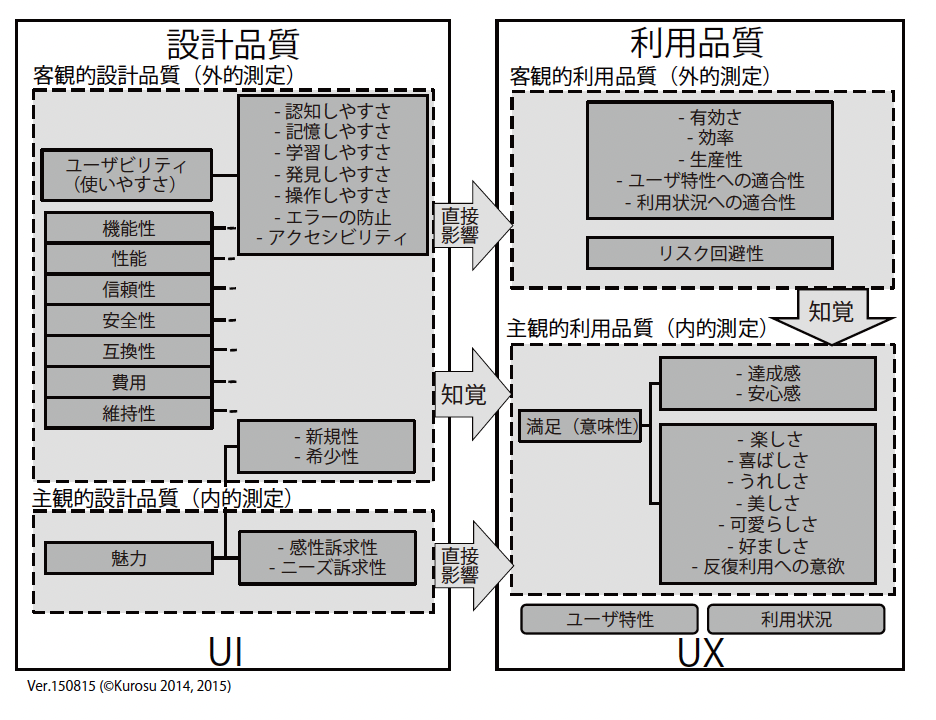
\includegraphics[width=100mm]{img/kurosu2015.png}
    \end{center}
    \caption{黒須の品質特性図\cite{kurosu}}
    \label{fig:kurosu2015}
  \end{minipage}
\end{figure}

このように,ユーザビリティ及びUXの評価はユーザにとって使いやすいシステムの開発に不可欠なものであり,その評価手法は定着しているもの,定着していないものを含めて様々に存在しているが,実際の開発ではUXの評価は大規模な消費者向けサービスを除いてほとんど行われていないか,行われていても改善に役立てられていないのが現状である.黒須\cite{kurosu}は,\begin{quotation}
  著者が企業における実態を調べると,そもそもUX調査を実施していることが稀というほど少なく,さらに実施していても,それを担当した部署と企画や分析を担当する部署との間の連携が取れておらず,せっかく取得した実利用に関する情報が企画やユーザ理解にもとづく具体化に役に立っていないことがわかった.
\end{quotation}と述べている.また,UX品質保証サービスを提供する企業が2020年にソフトウェア開発企業の社員490名を対象に行った調査では,UX向上に取り組んでいると応えた割合は34\%に留まっており,UXの評価を行っている割合は更に少ないと考えられる.実ユーザの体験を調査せずにユーザの満足性が高いシステムを開発することはできないため,小規模の開発でもUX評価を行えるようにする必要がある.

また,UXはユーザ毎に異なるだけでなく,使用の前,使用中,習熟後などのステージや折々の出来事によって変化するため,変化を考慮して評価する必要がある\cite{kurosu}.黒須はこのようなUXの変化を記述,視覚化するためにUXグラフ\cite{kurosu2015}を提案している.このUXグラフはユーザが製品を数週間から数ヶ月といった長期間にわたって使用した体験を,縦に満足性,横を時間軸にしてカーブで表すものである.一方で,システムを使用している数分間から1時間程度の期間の変化についてはユーザに変化を記述させることが難しくUXグラフは使われていない.しかし,UXの概念では,時間軸の変化は重要な要素であり,短期間の使用時であってもそれを評価する方法が必要であると考えられる.

以上のことから,(1)現在は大規模な開発でしか行われていないユーザテストの導入ハードルを下げ普及させること,(2)UXの重要な部分である満足性を測定する簡便な手法を開発すること,(3)(2)で測定した満足性からUXの時間変化を記録し可視化する手法を開発することが求められる.

%UXの説明が長い?
%UXがなんぞやよりも,UXの評価方法が無いことが問題
%1.1が長い

\section{目的}

本研究では(1)現在は大規模な開発でしか行われていないユーザテストの導入ハードルを下げ普及させるために,UX評価や統計処理についての専門的な知識が無くても容易にユーザテストを行いシステムの問題点を発見できるようにするシステムの開発を目指す.行動・生理メトリクスは確立された手法が無いため普及していないものの,分析の自動化と相性が良いため手法さえ確立できれば容易なユーザテスト手法になり得る.ユーザビリティテストでは,被験者は笑ったりそわそわしたり調査票に記入するよりもはるかに多くの行動を行うがそれらを記録することでより情報量の大きいデータを入手可能になる\cite{tullis2014}.そこで,(2)及び(3)の手法を用いて統合的な分析システムを開発する.

(2)満足性を測定する新たな簡便な手法として,容積脈波でストレスを測定する手法の満足性評価への応用を提案する.行動・生理メトリクスは満足性と関係があると考えられ,これまでにも皮膚伝導率や心拍数を用いてストレスで満足性を評価する手法が提案されてきた.容積脈波は,カオス解析することで鬱やパーキンソン病の診断に活用できる可能性が指摘されている\cite{tuan}\cite{oyama}.さらに,同様の解析により精神状態を測定できる可能性\cite{arai}が指摘されていることから,従来の皮膚伝導率や心拍数などのシンプルな方法よりも高精度なストレス測定が期待できる.また,脳波を用いてストレスを測定しユーザビリティを評価する手法\cite{amaral}も提案されているが,装置が大がかりになるために導入にコストがかかったり,測定器を装着すること自体がストレスになる可能性がある.そのため,耳朶に装着する小型のセンサーで容積脈波を取得しストレスを測定,満足性を評価する方法を提案する.これに基づき,容積脈波を解析して得たストレス指標と従来のユーザビリティ指標の関係を示した.

%UXグラフの画像

短期間のUX変化を黒須のUXグラフで表記させることは難しいが,容積脈波から得られるストレス指標のような生理メトリクスであればシーケンシャルであるため(3)使用中のUXの時間変化を記録し可視化することが可能になる.容積脈波を解析しストレスを算出するシステムであるLyspect\cite{oyama2012}では,ストレス指標の時系列変化を出力することができなかった.そこで容積脈波をリアルタイムで取得し,解析して得られるストレス変化を時系列グラフで表示するシステムを開発した.そして,開発したシステムの有効性を示した.

\section{本論文の構成}

本論文の構成を示す.

第\ref{chap:introduction}章では本研究の背景について述べた.第\ref{chap:prevresearch}章では関連研究と諸概念を整理する.第\ref{chap:pulsewave}章では脈波によるストレスチェックを応用したユーザビリティ評価手法を提案し,第\ref{chap:sequential}章ではそれを発展させた時系列ユーザビリティ評価手法を提案する.そして,それらの有効性を示す.最後に,第\ref{chap:conclusion}章の結論では本研究を総括し,考察と展望を述べる.付録として,本研究で行った実験で得られたデータを添付する.
  % 本文1
\chapter{関連研究と諸概念の整理}
\label{chap:prevresearch}

\section{ユーザビリティ}

\section{UX}

\subsection{時間相}

\section{満足性}

\section{UXメトリクス}

\section{指尖容積脈波}

ユーザテストでは,パフォーマンスメトリクスや自己申告メトリクス,行動・生理メトリクスを組み合わせて評価することが必要であると前に述べた.パフォーマンスメトリクスでは全ての部分を評価することはできないため,問題がありそうな部分や変更を加えようとする一部分のみを切り出して測定することになる.しかし,この計画立案についてもコストが高くなるため小規模な開発では実施が難しい.  % 本文2
\chapter{満足性と容積脈波から得るストレス指標との関係性}
\label{chap:pulsewave}

本章では,後述の時系列UX評価システムの開発に先立ち,容積脈波によるストレス指標と満足性の関連を把握するために行った予備実験について述べる.新たなストレス指標としては自律神経バランス(ANB)と最大リヤプノフ指数(LLE)を検討した.

\section{実験方法}

実験では,Nielsenのヒューリスティクスに基づいて作成した2つのUIを使ったタスクを被験者に実施してもらい,それぞれを使用している際のANBとLLEを比較した.ヒューリスティクスでBad UIとされているものは多くの場合満足性が低くなると考えられるものの,はユーザビリティ評価に使用するものであり,それがそのまま満足性に直結するとはいえない.そこで自己申告メトリクスを併用し,どちらのUIがより好ましかったかについて回答を求めた.

実験は2020年3月に17歳から74歳までの10名(男性8名,女性2名)を対象に行った.

\subsection{実験マテリアルの開発}

UX評価のマテリアルとして,Nielsenのヒューリスティクスで推奨されているUI(Good UI)と避けるべきとされているUI(Bad UI)を用意した.今回対象としたヒューリスティクスは``Visibility of system status'’(システムの状態の可視性)\cite{nielsen1990} である.10のヒューリスティクスのなかでアプリケーションの機能に関係ないものや学習が必要なもの,ユーザの予備知識に関係するものなど今回の実験に適さないものを排除して選択した.

具体的にはプログレス表示があるものをGood UI,無いものをBad UIとした.マテリアルの画面は図\ref{fig:old1}の通りである.画面にはノイズにならないように数字を表示するラベルと数字を変更するボタンのみを配置した.また,右上のスイッチでスタッフがGood UIとBad UIを切り替えられるようにした.アプリケーションの機能はNEXTボタンをタップするとランダムで0-5秒後にランダムな数字の表示が切り替わるだけのシンプルなものである.Good UIではNEXTボタンをタップすると図\ref{fig:old2}のようにプログレスを表示するインジケータが表示され,システムが次の数字を読み込み中であるという状態を表示する.一方でBad UIではNEXTボタンを押してもその時点では何の反応もなく,0-5秒後に数字が切り替わるまで上手くタップできたかどうかがわかりにくくなっている.

\begin{figure}[htbp]
  \begin{minipage}{0.5\hsize}
    \begin{center}
       \fbox{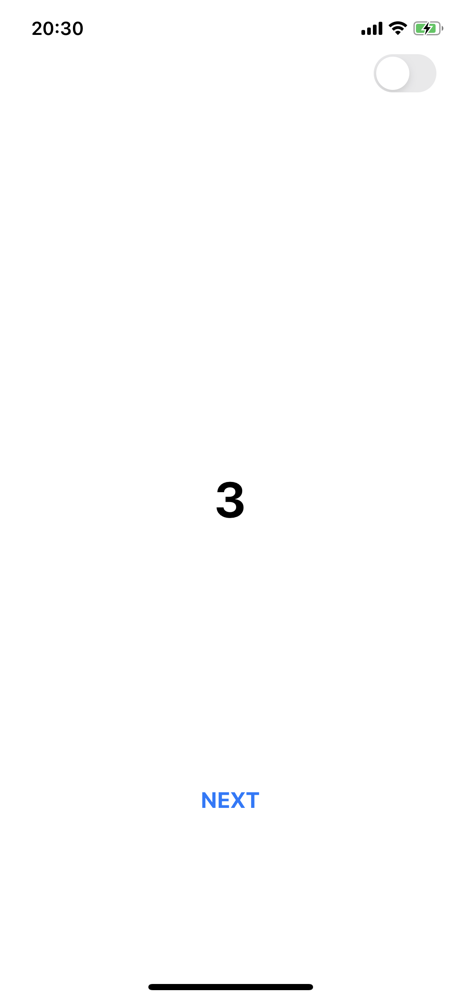
\includegraphics[width=40mm]{img/old1.png}}
    \end{center}
    \caption{実験マテリアル:数字の表示画面}
    \label{fig:old1}
  \end{minipage}
  \begin{minipage}{0.5\hsize}
    \begin{center}
       \fbox{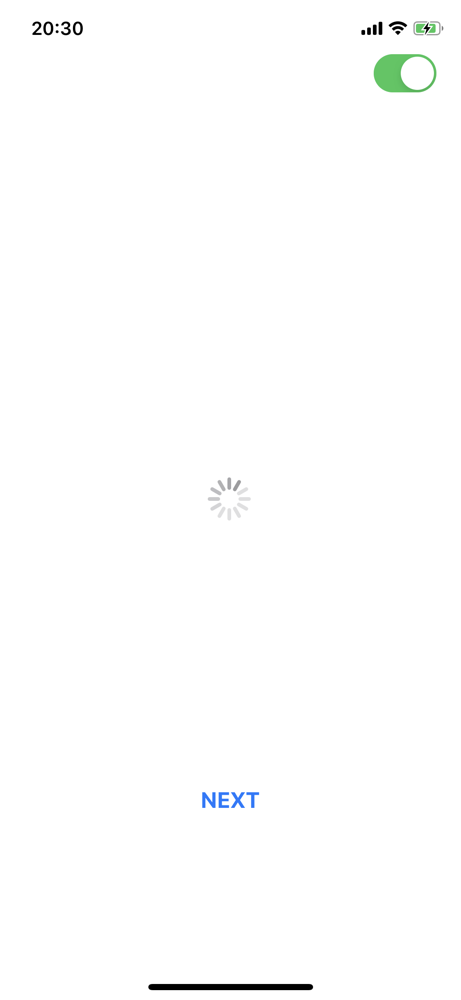
\includegraphics[width=40mm]{img/old2.png}}
    \end{center}
    \caption{実験マテリアル:数字の読込中画面}
    \label{fig:old2}
  \end{minipage}
\end{figure}

\subsection{タスクの実施}
被験者にマテリアルを操作してもらう際には,バイアスがかからないようにダミータスクを用意したうえでGood UIとBad UIそれぞれを順番に実施してもらった.なお,Good UIとBad UIの間には3分間の安静時間を設け,それぞれのマテリアルを操作する順番はカウンターバランスをとった.

ダミータスクは,1分間でNEXTボタンをタップして表示される数字をできるだけ多く書き取るものにした.できるだけ多く書くようにと指示することで,競争意識によって手を抜きにくくなるほか,早く表示してほしいと思わせるように設計した.

\begin{itembox}[l]{タスクの指示}
\begin{verbatim}
今から1分間のテストを2回行ってもらいます.このアプリでは,NEXTボタンを押すと数字が読み込まれますので紙に表示された数字を書いてください.書き終わったらもう一度NEXTボタンを押して次の数字を読み込んで紙に書いてください.制限時間は1分ですのでできるだけ沢山書くようにしてください.ただし,NEXTボタンを押してから数字が読み込まれるまで少し時間がかかりますので待ってください.
\end{verbatim}
\end{itembox}

\subsection{容積脈波(BVP)の計測}
BVPの計測は光学式指尖容積脈波計(PPG)のLifescore Quickプローブ(型番LQ-11,図\ref{fig:device2} )と専用の分析システムであるLyspect\cite{chaotechlyspect}を使用した.Lyspectでは300HzでBVPを記録し,LLEの平均とHF及びLFの値を取得した(図\ref{fig:lyspect}).被験者には実験の開始から終了まで利き手と逆の人差し指にセンサを装着してもらい休憩中も外さないようにした.なお,計測はマテリアルを使用している1分間の間のみとし1人当たり計2回記録した.


\begin{figure}[htbp]
  \begin{minipage}{\hsize}
    \begin{center}
       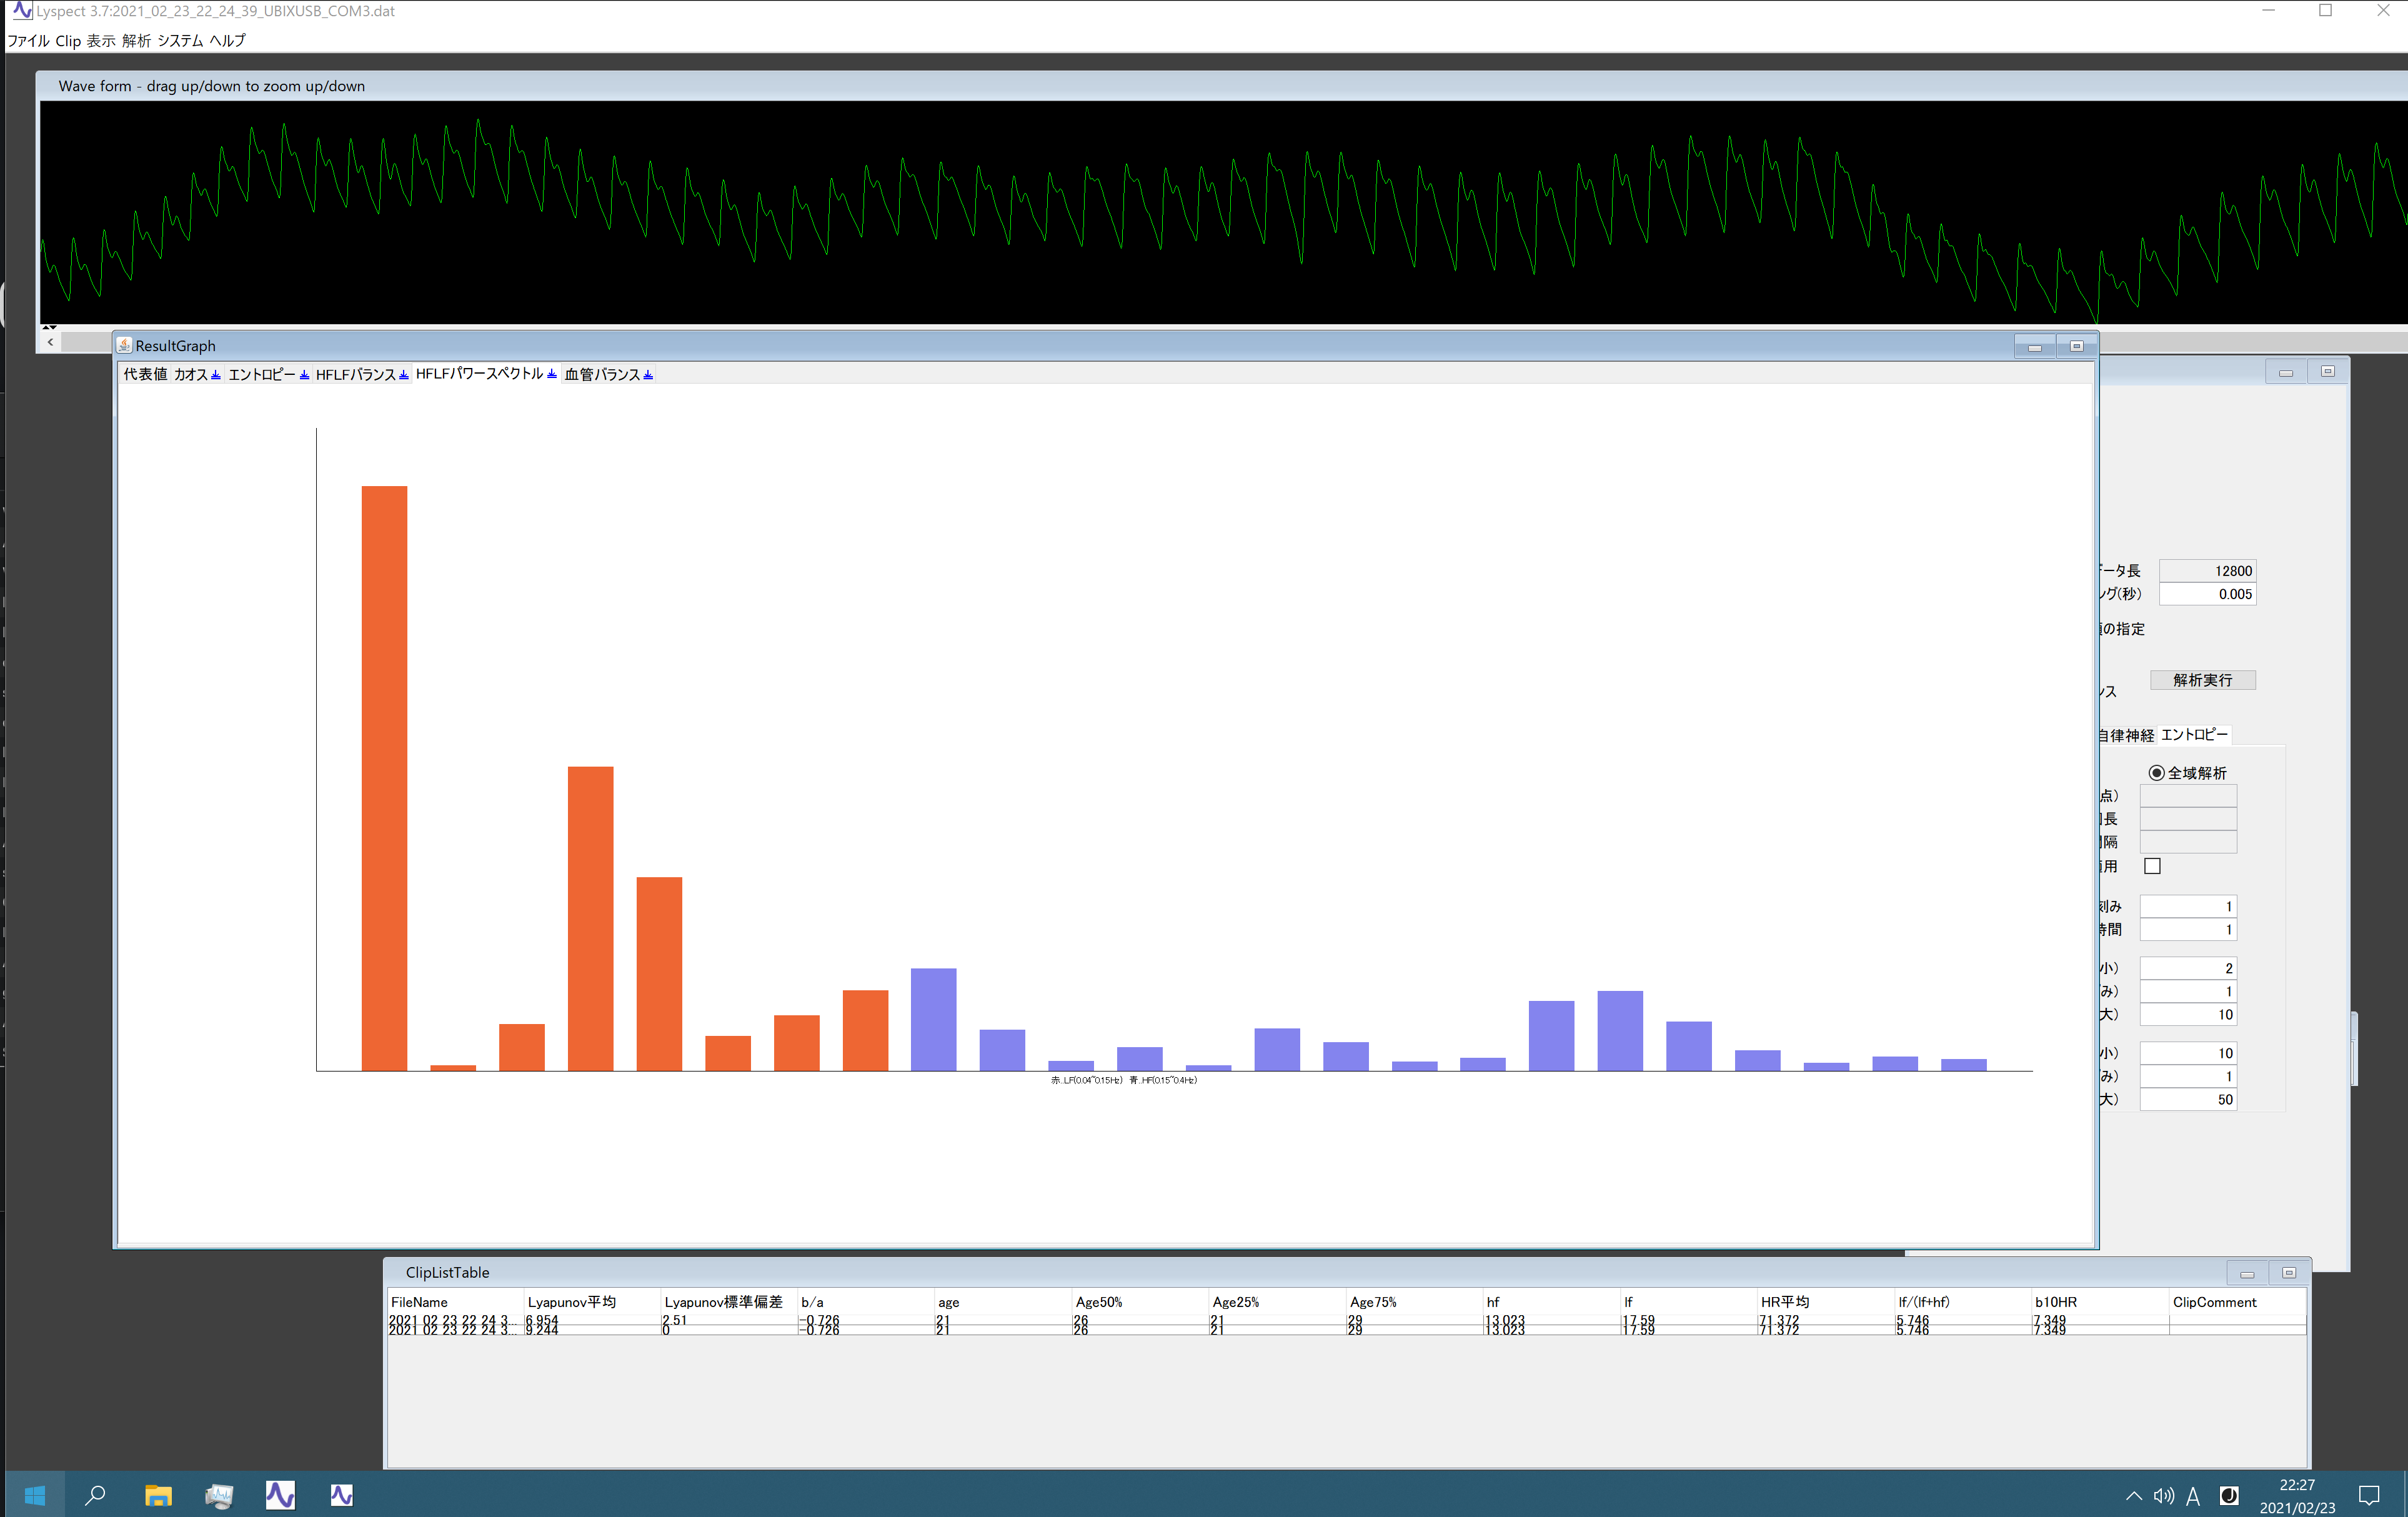
\includegraphics[width=100mm]{img/lyspect.png}
    \end{center}
    \caption{Lyspectでの分析画面}
    \label{fig:lyspect}
  \end{minipage}
\end{figure}


\section{結果}

\section{考察}

  % 本文3
\chapter{時系列UX評価システムの提案}
\label{chap:sequential}

\section{時系列UX評価システムの設計・開発}

\subsection{時系列ストレスグラフ}

\subsection{観察ビデオとのマッピング}

\section{有用性の調査方法}

\subsection{実験マテリアルの開発}

\begin{figure}[htbp]
  \begin{minipage}{0.5\hsize}
    \begin{center}
       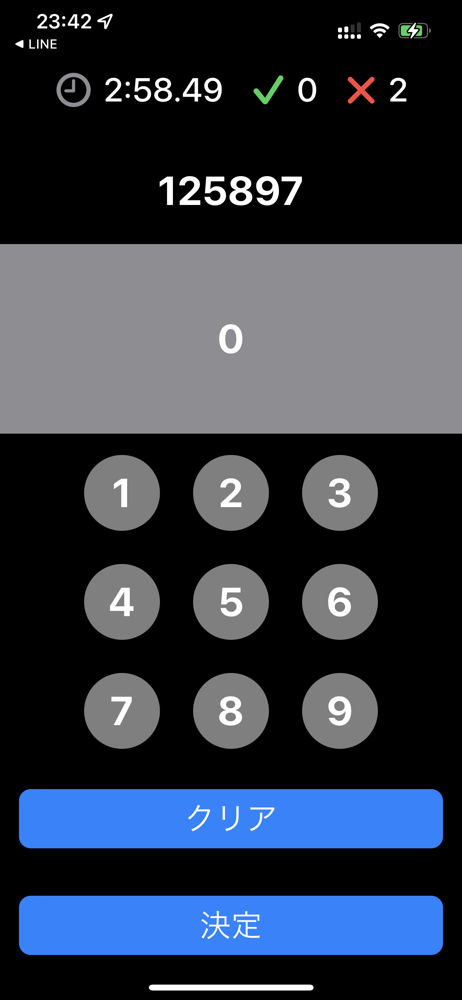
\includegraphics[width=40mm]{img/new1.png}
    \end{center}
    \caption{実験マテリアル:テンキー}
    \label{fig:tenkey}
  \end{minipage}
  \begin{minipage}{0.5\hsize}
    \begin{center}
       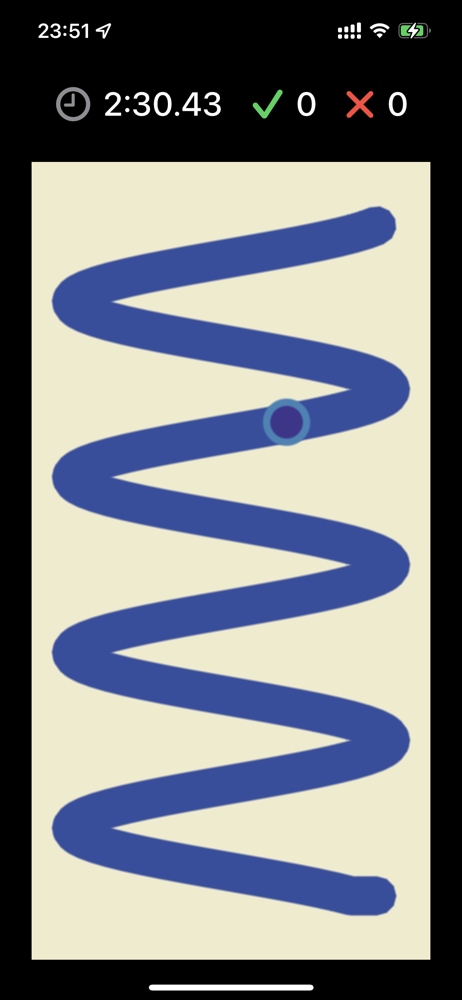
\includegraphics[width=40mm]{img/new2.png}
    \end{center}
    \caption{実験マテリアル:ドラッグ}
    \label{fig:drag}
  \end{minipage}
\end{figure}

\subsection{タスクの実施}

\subsection{容積脈波(BVP)の計測}

\begin{figure}[htbp]
  \begin{minipage}{\hsize}
    \begin{center}
       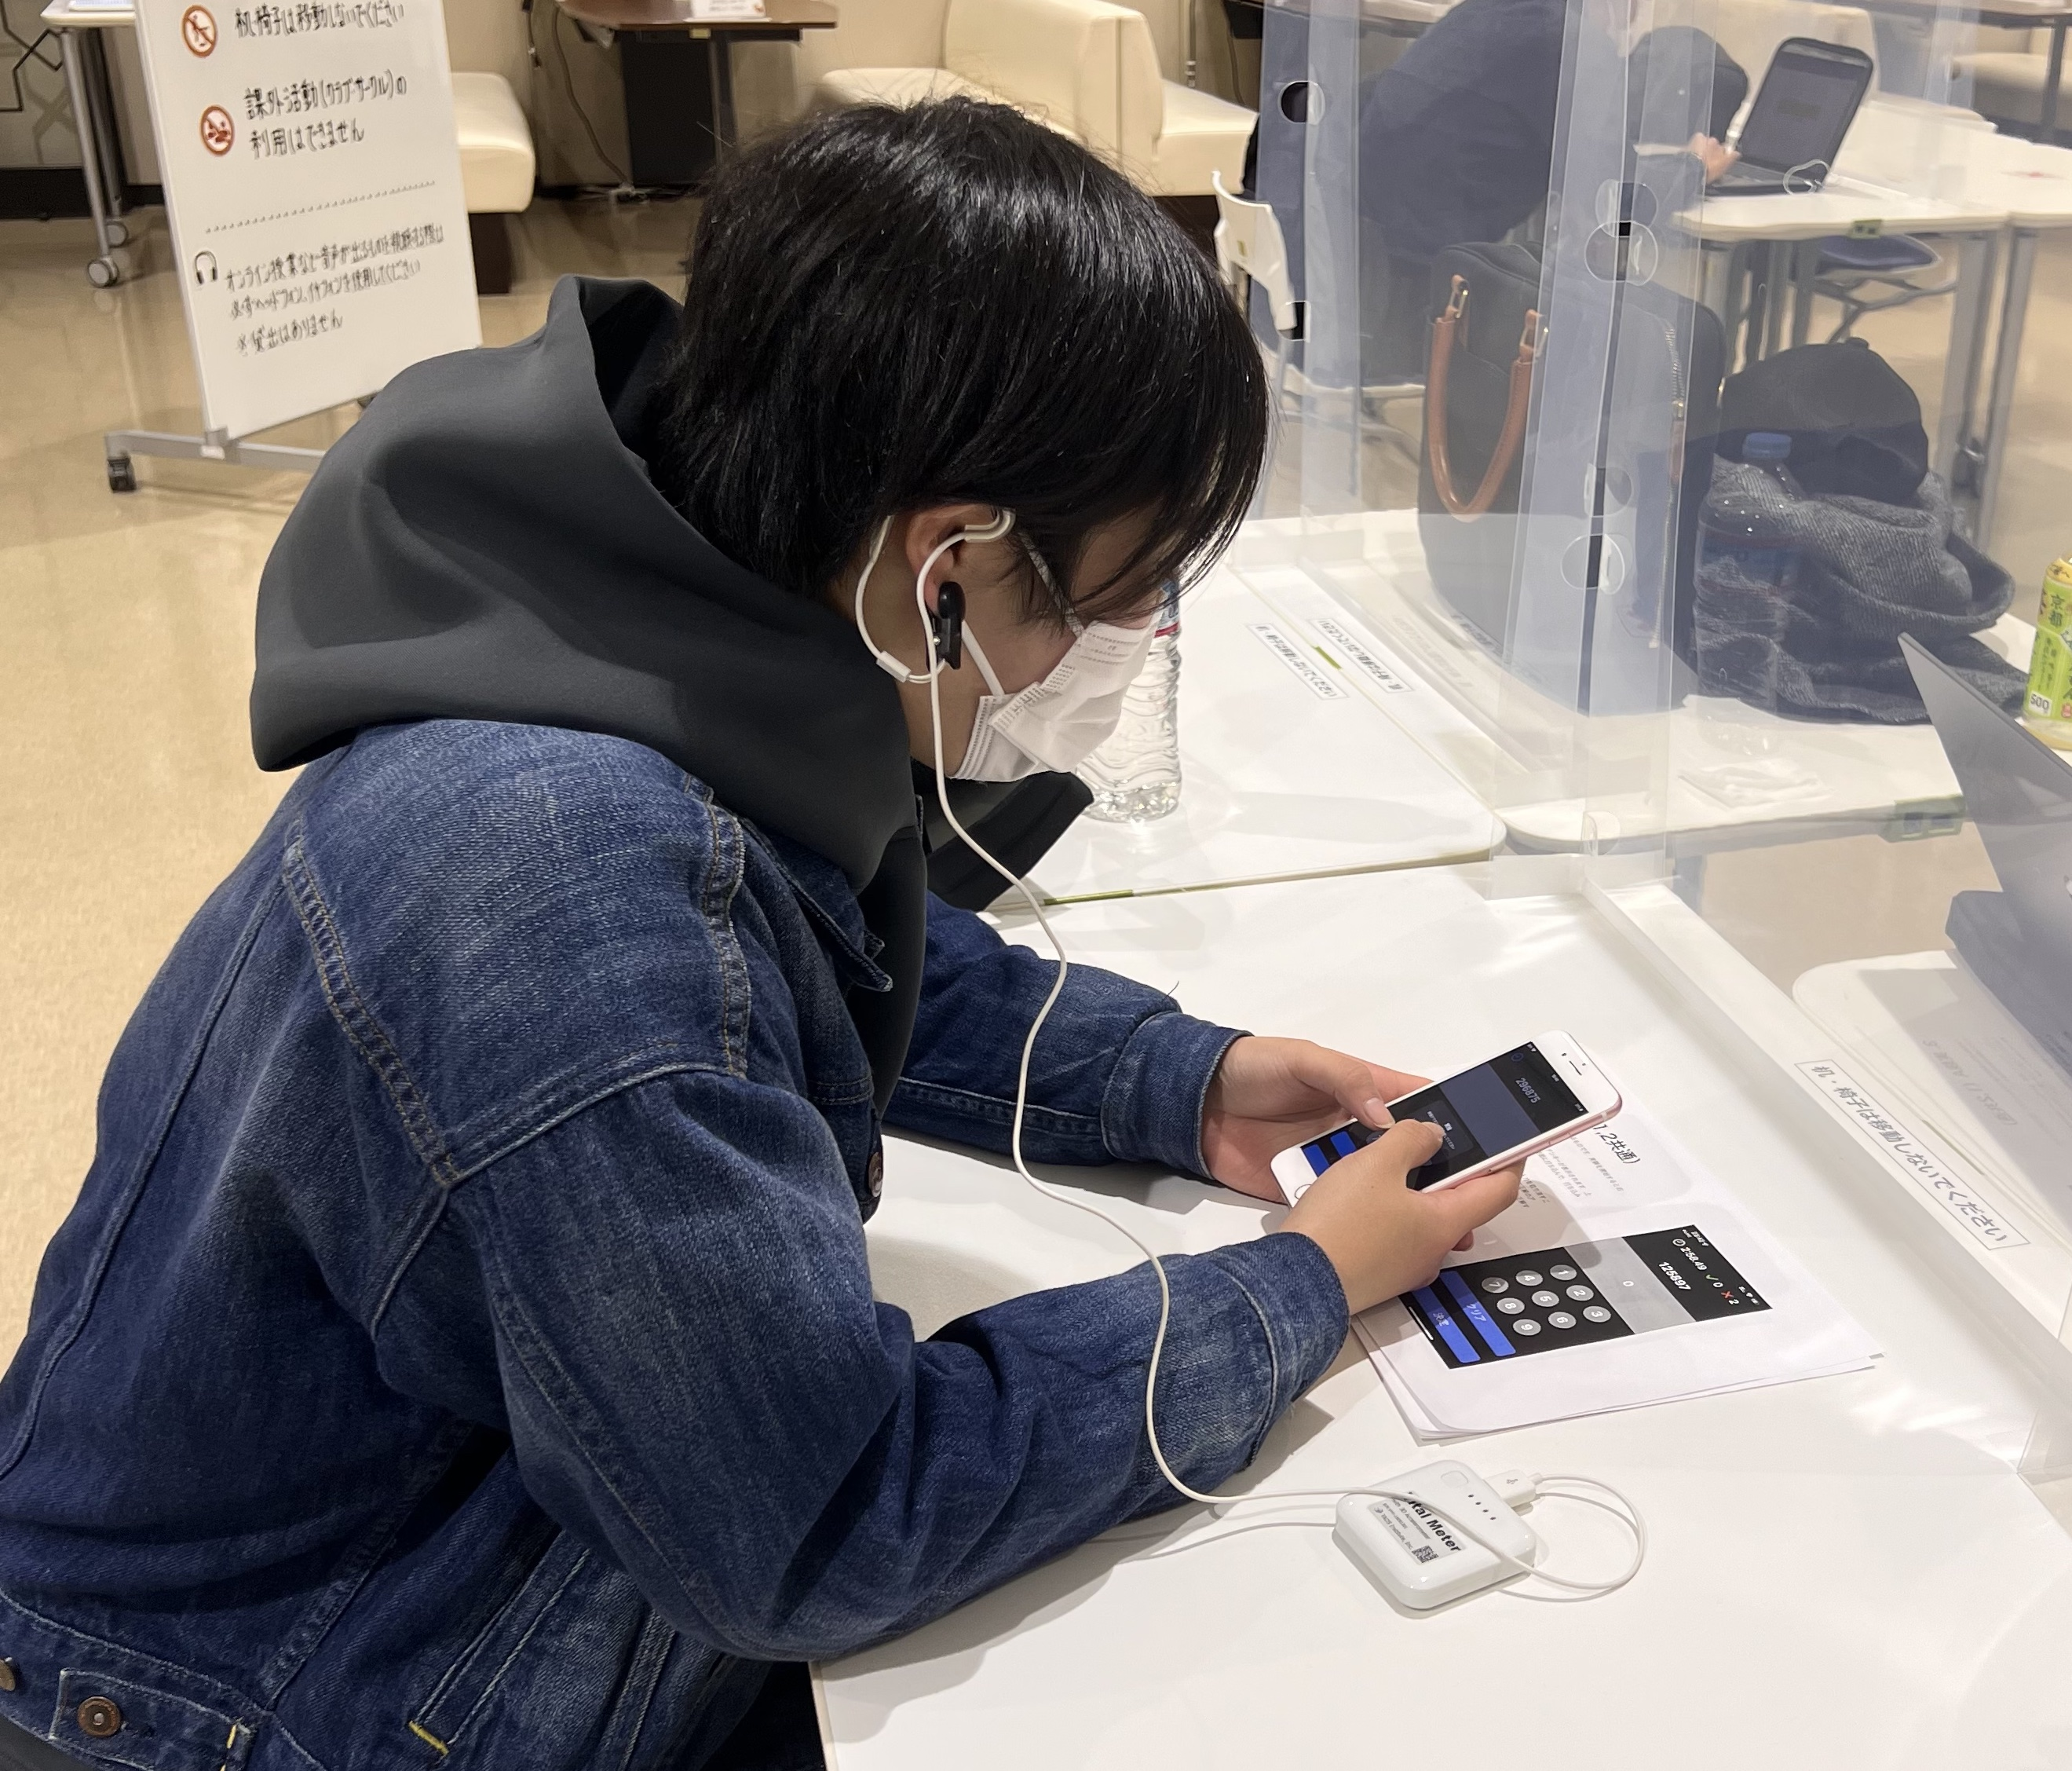
\includegraphics[width=100mm]{img/experience.jpg}
    \end{center}
    \caption{実験の様子}
    \label{fig:observe}
  \end{minipage}
\end{figure}

\subsection{アンケートの実施}

\section{実験の結果}

\section{実験の分析}

\begin{table}[htbp]
\centering
\begin{tabular}{llrlr}
\hline
    & \multicolumn{2}{l}{実験A}                             & \multicolumn{2}{l}{実験B}                             \\ \cline{2-5} 
    & Good UI(件)                & \multicolumn{1}{l}{Bad UI(件)} & Good UI(件)                & \multicolumn{1}{l}{Bad UI(件)} \\ \hline
肯定的 & \multicolumn{1}{r}{16} & 1                          & \multicolumn{1}{r}{22} & 3                          \\
否定的 & \multicolumn{1}{r}{}   & 34                         & \multicolumn{1}{r}{1}  & 34                         \\ \hline
\end{tabular}
\caption{アンケートの自由記述での否定・肯定意見の内訳}
\label{table:negaposi}
\end{table}

\begin{table}[htbp]
\centering
\begin{tabular}{lrrrrr}
\hline
            & \multicolumn{1}{l}{実験A}     & \multicolumn{1}{l}{}       & \multicolumn{1}{l}{実験B}     & \multicolumn{1}{l}{}       & \multicolumn{1}{l}{\multirow{2}{*}{合計(件)}} \\ \cline{2-5}
            & \multicolumn{1}{l}{Good UI(件)} & \multicolumn{1}{l}{Bad UI(件)} & \multicolumn{1}{l}{Good UI(件)} & \multicolumn{1}{l}{Bad UI(件)} & \multicolumn{1}{l}{}                    \\ \hline
スムーズ        & 7                           &                            & 8                           &                            & 15                                      \\
反応が良い       & 3                           &                            & 5                           &                            & 8                                       \\
快適だった       & 3                           &                            & 5                           &                            & 8                                       \\
正常だった       & 2                           &                            & 1                           &                            & 3                                       \\
ゲーム性があった    &                             & 1                          &                             & 1                          & 2                                       \\
達成感があった     &                             &                            &                             & 2                          & 2                                       \\
順調だった       &                             &                            & 2                           &                            & 2                                       \\
ストレスを感じなかった & 1                           &                            & 1                           &                            & 2                                       \\
挑戦したくなった    & 1                           &                            &                             &                            & 1                                       \\
ミスが無かった     &                             &                            & 1                           &                            & 1                                       \\
多く正解できた     & 1                           &                            &                             &                            & 1                                       \\
楽しかった       & 1                           &                            &                             &                            & 1                                       \\ \hline
\end{tabular}
\caption{アンケートの自由記述での肯定的意見の内訳}
\label{table:posi}
\end{table}

\begin{table}[htbp]
\centering
\begin{tabular}{lrrrrr}
\hline
             & \multicolumn{1}{l}{実験A}     & \multicolumn{1}{l}{}       & \multicolumn{1}{l}{実験B}     & \multicolumn{1}{l}{}       & \multicolumn{1}{l}{\multirow{2}{*}{合計(件)}} \\ \cline{2-5}
             & \multicolumn{1}{l}{Good UI(件)} & \multicolumn{1}{l}{Bad UI(件)} & \multicolumn{1}{l}{Good UI(件)} & \multicolumn{1}{l}{Bad UI(件)} & \multicolumn{1}{l}{}                    \\ \hline
反応が悪かった      &                             & 25                         &                             & 23                         & 48                                      \\
難しかった        &                             & 4                          &                             & 8                          & 12                                      \\
ストレスを感じた     &                             & 5                          &                             & 5                          & 10                                      \\
ミスがあった       &                             & 8                          &                             & 2                          & 10                                      \\
焦った          &                             & 6                          &                             & 1                          & 7                                       \\
悔しかった        &                             &                            &                             & 5                          & 5                                       \\
作業のように感じた    &                             &                            & 1                           & 1                          & 2                                       \\
動揺した         &                             & 2                          &                             &                            & 2                                       \\
煩わしかった       &                             & 1                          &                             & 1                          & 2                                       \\
モヤモヤした       &                             &                            &                             & 1                          & 1                                       \\
何がダメかわからなかった &                             &                            &                             & 1                          & 1                                       \\
困った          &                             &                            &                             & 1                          & 1                                       \\
慣れなかった       &                             & 1                          &                             &                            & 1                                       \\
疲労を感じた       &                             &                            &                             & 1                          & 1                                      \\ \hline
\end{tabular}
\caption{アンケートの自由記述での否定的意見の内訳}
\label{table:nega}
\end{table}


\section{実験の考察}

  % 本文4
\chapter{結論}
\label{chap:conclusion}

\section{満足性評価のための指標}

第\ref{chap:pulsewave}章では新たな満足性評価指標としてANBとLLEを提案し,次の結果が得られた.

\begin{enumerate}
\setlength{\parskip}{0cm}
  \setlength{\itemsep}{0cm}
  \item ANBは満足性が高いUIを使用したときと低いUIを使用したときとの間で有意な差が見られ,満足性が高いUIを使用したときのほうが低くなる傾向が見られた.
  \item LLE及びHRでは有意な差が見られなかった.
\end{enumerate}

(1)ANBは満足性の評価指標として,UX評価に有用である可能性が示唆された.また,いまだ手法が確立されていないUX評価において,UXの重要な概念のひとつである満足性を定量的に評価する新たな手法としてPPGを用いたBVPの測定とANBの活用を提案した.

(2)従来研究用途で活用されることがあったHRは用途や測定方法によっては活用が難しい可能性を指摘した.LLEについては,数分レベルのまとまった時間の代表値としてUX評価に利用することは難しいことが明らかになった.

\section{時系列UX評価システム}

時系列UX評価システムとして,ANB,LLE,RRIを十数秒から数分程度の短いスパンで区切り一定秒毎にスライドさせながら繰り返し計算することで時系列でそれらの値を取得できるようにするシステムを開発した.また,実施時の状況を記録した動画やスクリーンキャプチャを脈波と同期させることでどのようなアクションを行った際にストレス指標が変化したのかを表示できるようにした.

システムの有用性を調査するために行った実験では,使用中に各指標の変化があったものの,Good UIとBad UIの間でのストレス指標の変化を明確に示すことができなかった.

\section{今後の課題}

本研究では,PPGとANBの活用の可能性をしめすことができた.一方で残されている課題について述べる.

第\ref{chap:pulsewave}章で行った実験では,ANBの有用性が示唆された.しかし,実験で用いたBad UIの例は限られており,繊細なUIの差異に代表されるような様々なUIの問題点を検出できるかどうか検討する必要がある.これにより,実際の開発においてANBがどこまで信頼できるのかを明らかにできると考える.

時系列UX評価システムはプロトタイプであるため実用上の課題があり,改善していく必要がある.まず,BVPと動画をそれぞれ別に記録し後からシステムに読み込むのではなくシステム上で一元的に記録できるようにする必要がある.同時に,自動的にBVP,動画の同期を行うようにすることでより同期精度を高め正確な測定が可能になる.次に,入力したBVPのエラー処理を改善する必要がある.現時点ではBVPは目視でセンサーのずれによるノイズが無いかどうかを確認しているが,見落としをなくし簡便にするためには機械学習を用いて自動的に削除する仕組みが必要である.以上のような改善を通じてより正確なストレス評価を可能にする必要がある.

今回の実験では,各操作時のストレス指標の変化をグラフ化したものの,その解釈に検討の余地があった.今回のように,実験毎の分析ではなく,タップなどの操作レベルで変化を分析する必要がある.さらに,操作によって生じたストレス変化が指標に反映されるまでの時間についても検討する必要がある.

\subsection{統合的なシステムとしての展望}

本システムは,今後統合的なUX評価システムとして発展させたいと考えている.その内容について述べる.

システムはBVPを測定する画面(図\ref{fig:futurework1},\ref{fig:futurework2}),被験者毎に分析する画面(図\ref{fig:futurework3}),複数の被験者をまとめてそのストレス変化を画面遷移図の上に表示する画面(\ref{fig:futurework4})で構成される.

測定画面では,今回開発したシステムが備える動画とBVPの同期に加えて発言や操作ログなど様々な満足性指標を記録できるようにする.そして,分析画面で被験者を個別に分析し,そのデータを集約して画面遷移図上にストレスが高いと感じている被験者が多い部分を表示する.

このシステムによって,UX評価が誰でも簡単に実施できるようになる.さらにユーザの個別の反応であるUXを,複数人分まとめて画面遷移図上に可視化することで製品設計に落とし込むところまでを補助できるようにすることを目指している.

\begin{figure}[htbp]
  \begin{minipage}{0.5\hsize}
    \begin{center}
       \includegraphics[width=70mm]{img/design_record_1}
    \end{center}
    \caption{測定画面のプロトタイプ(アプリ用)}
    \label{fig:futurework1}
  \end{minipage}
    \begin{minipage}{0.5\hsize}
    \begin{center}
       \includegraphics[width=70mm]{img/design_record_2}
    \end{center}
    \caption{測定画面のプロトタイプ(VR用)}
    \label{fig:futurework2}
  \end{minipage}
\end{figure}


\begin{figure}[htbp]
  \begin{minipage}{\hsize}
    \begin{center}
       \includegraphics[width=100mm]{img/design_analyze}
    \end{center}
    \caption{分析画面のプロトタイプ}
    \label{fig:futurework3}
  \end{minipage}
\end{figure}

\begin{figure}[htbp]
  \begin{minipage}{\hsize}
    \begin{center}
       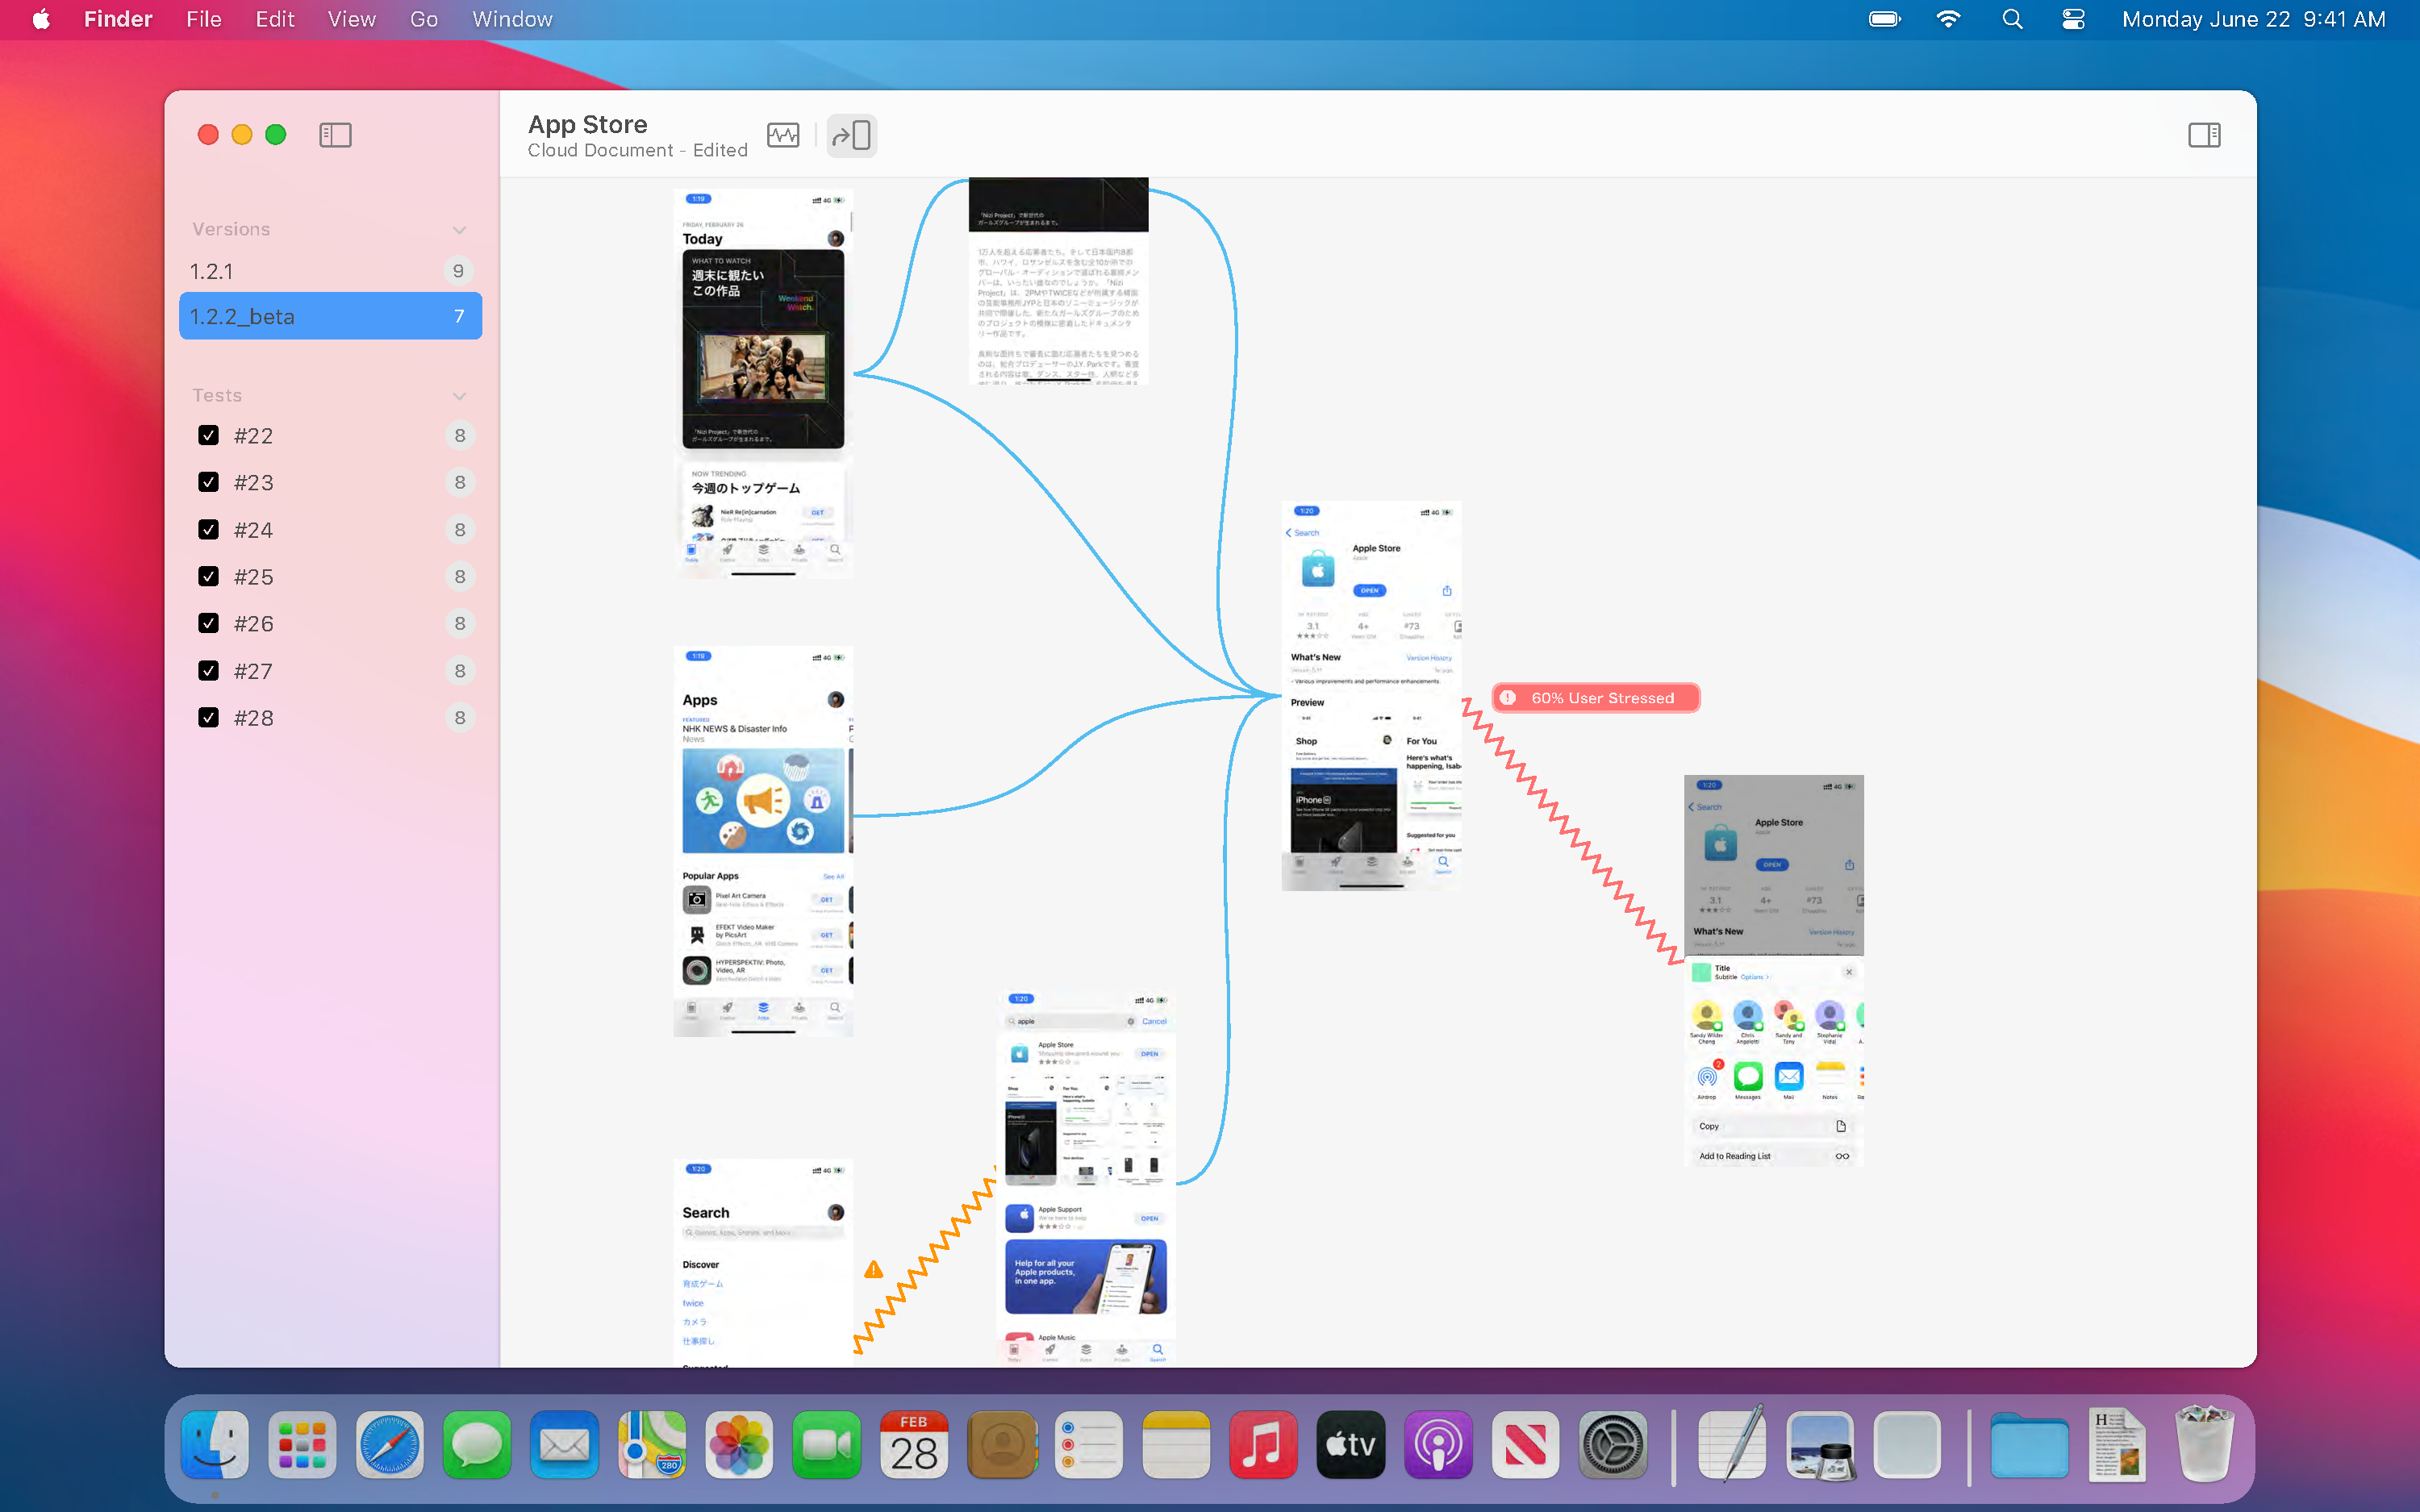
\includegraphics[width=100mm]{img/design_storyboard}
    \end{center}
    \caption{画面遷移図での可視化画面のプロトタイプ}
    \label{fig:futurework4}
  \end{minipage}
\end{figure}
  % 本文5

\begin{acknowledgment}

本研究は,孫正義育英財団の支援を受けて実施されたものです.

\end{acknowledgment}
  % 謝辞。要独自コマンド、include先参照のこと

\begin{bib}[100]
% BibTeXを使う場合
\bibliography{main}

%\begin{thebibliography}{#1}
%
%  \bibitem{参照用名称}
%    著者名: 
%    \newblock 文献名,
%    \newblock 書誌情報,出版年.
%
% \bibitem{hoge09}
%   ほげ山太郎,ほげ山次郎:
%   \newblock ほげほげ理論のHCI分野への応用,
%   \newblock ほげほげ学会論文誌,Vol.31,No.3,pp.194-201,2009.
% 
% \bibitem{hoge08}
%   Taro Hogeyama, Jiro Hogeyama:
%   \newblock The Theory of Hoge,
%   \newblock {\it The Proceedings of The Hoge Society}, 2008.
%	
%\end{thebibliography}

\end{bib}
  % 参考文献。要独自コマンド、include先参照のこと
\appendix
\chapter{付録の例}

付録を無理矢理出力させるため、てきとうなことを書く。

\section{ほげ}

コマンドは本文と一緒。

\subsection{ふー}

本文と一緒。

\section{ほげほげ}

本文と一緒。

\subsection{ふーふー}

本文と一緒。
    % 付録
\chapter{時系列UX評価システムの妥当性調査実験 自由回答}

\section{実験A}

\begin{itemize}
  \item どちらも正解だと思った答えを入力しても、正解にならなかったのは不思議だと思いました。1回目の方は入力するたびに焦りとイラつきがありましたが、2回目の方はずっと不正解でも何度もトライしようという気になりました。
  \item 1回目の実験のとき、何度タップしても反応がなかったので、少し焦った。
  \item 1回目について、まず初めに入力したはずの数字が入力されず、困惑した。そのあと何回かランダムに押せば入力すればいいと気づくも、課題通りに入力したはずなのに不正解となり、始めに聞いた課題を書き間違えたのかと思って焦った。何回か小さい順から入力後、違うアルゴリズムで正解になるパターンだと考え、大きい順から入力するも不正解となり、表示されたまま入力すると正解したので意図を理解した。1回目はその理解までに1分半くらいは使ったと思う。誤入力もありストレスだった。2回目は念のため言われた通りの課題をこなしたが不正解となったので、そのまま入力するのに徹した。タップしたらそのまま数字が入力されるので快適だった。
  \item 1回目ではテンキーの入力判定が悪く、2回目では普段利用している時と変わらない判定であった。
  \item "1回目はボタンの感度が悪く、6回押さないと数字が入力できないときがあったが、2回目は一回押しただけでボタンが反応した.スマホの反応の速さの違いによる感情の変化を調べる実験だったのか?"
  \item 2回目の数字が押しにくかったです。
  \item 素直に反応してくれないとイライラする
  \item 1回目のときは、スムーズに数字を当てたが、2回目のときは、何度押しても反応しない時があったので動揺しました。
  \item クリアボタンの位置が悪魔的
  \item はじめは反応悪いだけかなと思ったけど、ひとつ前の実験から察するに、「そういうやつね」となった。
  \item 1回目の実験では1度のタップで反応しない場合もあったため、入力に煩わしさ対して2回目の実験では全ての操作が1度のタップで行えたためスムーズな入力感だった。
  \item 1回目に行った時は数字の打ち込みがとても難しく、スマホの画面に問題があるのではないかと思うほど打ち込みにくかった。しかし、2回目はとてもスムーズにいつもスマホを触る時と同じように打ち込むことができた。
  \item 先にスムーズに操作できる回からだったため、2回目の異常さにはすぐに気がつきました。初めは、わざととは思わず、何か実験に不備が出てしまうのではないかと心配になりました。スムーズに操作できないと、押し間違いのミスをしてしまった時のあっ。という気持ちが大きくなり、自分の焦りに繋がるように思いました。2回目の方が、スピードよりも正確性重視で操作を行なっていたように思いますし、小さなストレスも多かったと感じます。
  \item  2回目に数字を入力するのが、うまく行く場合と行かない場合が不規則だったので、最後までなれなかった。
  \item 1回目はスムーズに入力できたのに対して、2回目はとても押し辛かったです。
  \item 2回目の方が反応がよかった。1回目の方は何回も数字を押さないと反応しなかった。
  \item タップした時に自分が思ったように数字を押せていなかったら焦ってミスが生まれた。また、何回も繰り返していくと最初より精度が落ちた気がした。
  \item 2度目はテンキーの反応が悪く苛立ちがあったため、クリア・決定の操作も誤ることがあった
  \item 2回目の方が入力しづらかった。
  \item 1回目の何度も押さないといけない方は、煩わしかった。
  \item 2回目の時に一度数字を選択しても反映されなくて、連打しているうちに2回押しちゃってまた1番最初からやり直しということが何回かあって、少し焦った。
  \item 1度目は何度か押しても反応しない場合があった2度目はスムーズに行けた
  \item 1回目は数字のボタンが押しにくく何回も入力し直した。2回目はスムーズに入力できストレスフリーで行うことができた。
  \item 1回目に数字を押した時は反応しづらかった.直前のアンケートでは普通に反応していたため、何かそういうアプリかなあと思いました2回目は普通に打てたので楽しかったです
  \item 初めの方は動きが悪くて、やりづらいなと思いました。
  \item 1回目の実験で入力する際に、押しても反応しない時があったのがとてもいらいらしました。2回目は押しやすかったです。
  \item 一回目の実験の操作は、数字ボタンが反応しないことがあり難しかった。しかし、クリアと決定ボタンには不具合がないのが不思議だった。二回目の実験の操作は正常に反応したため快適に感じた。
  \item 2回目の実験の際に、ボタンの反応が悪くなり、入力ミスを起こしてしまった。
  \item 1回目は一度入力すれば文字が反映されたのに対し、2回目はランダムで1〜5回タップしないと文字が反映されなかった
  \item バラバラに数字を並べられると意外と難しい。2回目はわざと一発で入力できないようにされているのだなと感じた。自分のめんどくさがりで短気なところから何回もタップして同じ数字を2回入力してしまったりした。単純にゲーム感覚で面白かった。
  \item 1回目の実験ではレスポンスが早く感じたが2回目の実験ではレスポンス以前の問題で数回押してもなぜか反応しないことがあったため意図的に反応させないとしたら結構悪用が可能なのではと考えている。
  \item 2回目では画面の反応が悪くストレスを感じた。また、なぜか問題解答の正確さも落ちてしまった。
  \item 1回目は普通だったけれど、2回目は数回に1回だけ反応していた。
  \item 1回目は数字が打ちづらかった。
  \item 一度目は反応が鈍く反映されにくく、二度目は普通に押せば反映されるように感じた
  \item 入力のしやすさに差があった。
  \item 2回目の実験は入力しづらかった。
  \item 1回目の時は少し反応が鈍かったので、2回目の時の方が多く正解することが出来ました。
  \item 2回目にストレスがかかるように設計されたゲームであると気づいた。反応が悪いほうをするときの方が慎重になってゲームしていた気がする。反応しないと思って連打するときもあったためミスも増えたように感じた。
  \item 1回目は何度かタップしないと文字入力ができなかった。2回目はスムーズにできた。
  \item 初め、文字が打ちにくくて機械の不具合かと思った。
  \item 6つの数字を、3つずつに分けて考えると素早く判断することができると感じた。何回か繰り返して慣れてくると、逆に入力ミスや小さい数字の見落としなどのミスが増えてきたように感じた。
  \item 数字のボタンを押しても反応しないことがある。
  \item ・1.2回目共、数字のキーをなぞるように打っていくとミスが少ないと感じ、そのように行った。・1回目と比較して2回目では数字を打つのが難しく、その分ミスタッチが多くなったため慎重に行う方がいいと判断し、そうした
  \item 2回目は1回目と違って、テンキーが反応しない時があった。

\end{itemize}

\section{実験B}

\begin{itemize}
  \item 1回目の方は時間内に1回だけしかクリア出来なかったので、ゲーム性があって面白かった。2回目の方はスムーズに操作できたが、何をしてもクリアしたので、ゲーム感覚よりかは作業のように感じた。
  \item 2回目の実験のとき、ボールが思ったように動かなかった。半分以上進んだときにやり直しになったときは、少し悲しかった。
  \item 数字の入力を経験した後なので1回目のボールの実験も面倒なやつだろうなと思って取り組んだ。最後まで行けなかったのが悔しい。2回目はとても快適だった。
  \item 1回目ではボールを動かす際の移動距離はランダムであるような気がした。2回目では指の動きとボールの動きがリンクしており、ゴールが容易であった。また、2回目でははみ出した判定が線に対してボールの1番離れた所となっていた。
  \item 1回目は指でなぞった通りにボールが動いたが、2回目はボールの動きを操れなかった。スマホの反応の速さの違いによる感情の違いを調べる実験なのか?
  \item 一回目が楽だったので、二回目はめんどくさくなると予測していたが想像以上だったので、かなりのストレスだった。
  \item 1度目のものは何がだめで振り出しに戻されてるのかわからなかったです。2回目もなぜ戻されているのかわかりませんでしたが、スムーズに動く分やりやすかったと思います。
  \item 2回目反応が悪く球を動かしにくかった
  \item ひたすら同じことを繰り返すと飽きてくる。
  \item 1回目のときは、なかなかボールが動かなくて困りましたが、2回目のときはスムーズに動くようになったので一瞬さっきの動かし方が悪かったのかと思いました。
  \item 2回目が特に難しい
  \item はじめは反応悪いだけかなと思ったけど、時間が経っても改善されないので「そういつやつね」となった。1回目が順調だっただけに、2回目が一回も成功できずモヤモヤした。
  \item 1回目の実験では指での入力に対して不自然な反応だったため、少しいらだちを感じて1度しか成功しなかった。対して2回目の実験では、入力に対して素直な反応だったため、成功回数が一回目に比べて多くなった。
  \item 数字を打ち込む作業と同じくとてもやりづらく、指先を繰り返し小刻みになぞる動作だった。とてももどかしく感じた。2回目はなぞることがとても楽で、あまり神経質にならずにスピードを速めながらなぞることができた。
  \item 先に、上手く操作ができない回からおこなったため、この感度が正常なのかと無理やり思い込んで頑張ろうとしていたように思います。そのため、うまく操作できない自分への焦りを感じました。身近な機器がスムーズに操作ができることは、勉強や自由時間のクオリティを格段に上げてくれていることを実感したように思います。
  \item 1回目は、あまりにもタッチの反応が悪かったので、最後までうまく行く方法がわからなかった。2回目は1回目と比べて驚くほど反応が甘かった。
  \item 一回目全くボールが動かなくて、最初の坂で止まってしまった。2回目はスムーズでやりやすかった。
  \item 1回目の方が2回目よりも反応が良かった。しかし、どちらも数字なら実験に比べると反応が悪かった気がした。
  \item こちらも、最初の方はすぐにゴール出来たが、繰り返していくうちに思った位置までボールがきていないことが増えミスが増えた。一回ミスすると繰り返してしまった
  \item 2回目は反応が悪く思った通りに動かなかったがむしろ集中できた
  \item 2回目の方が反応が悪く、1回もクリアできなくて残念だった。
  \item 携帯が、ちゃんと思い通りに動いているのは、嬉しい。感謝の気持ちが芽生えた。
  \item 1回目は一度もミスすることなく何回も成功できたが、2回目は全然指に合わせてボールが動かなくて少しイライラした。一度は成功できたものの、他はすぐに一番最初からになったので悔しかった。
  \item 1度目は進むスピードが遅く、少しのズレで最初からのやり直しだったため、難しかった
  \item 1回目はスムーズにボールを動かすことができ、はみ出してもまたやり直せばいいという考えから素早く操作できたが、2回目は動かしにくかったため慎重に動かしすぎて時間内にゴールまで辿り着けなかった。
  \item 数字の方と交互にやったため、2回目は触りやすくなってるのかなと寧ろ3分間あの単調な作業をする方が頭おかしくなりそうです
  \item 初めの方は一筆ではかけず、2回目はスイスイかくことができました。
  \item 2回目の実験で、ボールをうまく進められなかったり、なんとかして進めようとしたが最初に戻ったりして、とてもイライラしました。1回目はスムーズにできました。
  \item 一回目の実験の操作は、なぞった際に進む速度がバラバラで難しかった。また、途中でボールの上に指を合わせる必要がないことに気づいた。二回目の実験の操作は、ボールの上をなぞった通りに動いたため快適だった。一回目よりもアウト判定がゆるいように感じた。
  \item 1回目の実験ではボールの反応が悪かったものの、2回目では回復したため、少し驚いた。
  \item 1回目はスムーズにすらすらとボールが動いたのに対し、2回目は徐々にしか動かず、1回目よりも2回目の方が「線から外れた判定」が厳しいと感じた
  \item ボールをスライドさせるという説明文では指をボールに置くのか進行方向に指を動かすのかわからなかった。一回目は非常にカクカクしていてやりづらかった。これは数字と反対でわざと一回目がやりづらくされていたと気づいた。一回目がカーブのところでコースアウトしてしまったのでスムーズに動く二回目でも慎重になった。
  \item 一回目は明らかにレスポンスが悪く実験どころではない状況であった。ゲームであれをやられたらレビューが悲惨なことになること間違いなしである。2回目は大凡のレスポンスが改善されておりあの動作ならまだ問題ないと思う。
  \item 2回目では思った通りにボールが動かずより正確になぞれるように注意した。一回しかうまくいかなかったがうまく行った時は達成感を感じた。
  \item 一回目は普通だったけれど、2回目は滑りづらくて、私の手が人間じゃなくなったのかとおもった。そういう実験なのかなぁどっちなのかなあと思っていたら2回目の数字もへんだったからそういう実験なのだなと思った。
  \item 1回目はボールが動かしづらかった。
  \item 一度目は有効な範囲が狭く、触っても反応しているかわからないようなほどしか進まなかったが、二度目はさらさら出来たため、どこまではみ出して動かしてもいいか試したりしながら進めた。だいぶはまだしても大丈夫だったように感じた。
  \item 2回目の実験が動かし易かった。
  \item 1回目の実験はなぞりにくかった。
  \item 1回目はボールが少しずつしか進まなかったので、2回目の方がスムーズに行うことができました。
  \item 1回目の方がボールの反応が悪く自分が思った通りに動かなくストレスがあった。2回目と比べした後の疲労感という意味でも1回目の方がしんどかった。1回目は1回もクリアできていなかったため、最後になればなるほど焦りが出てきてまたミスも増えたのかもしれない
  \item ボールが1回目に比べてとても動かしにくかった。少しでもずれると最初に戻ってしまうので難しかった。
  \item 二回目はボールが動きづらくなっていたため、非常にやりづらく、多少の苛立ちがあった。
  \item コツを掴むと素早くなぞることができたが、一度変な癖がついてしまって何回か連続してミスしてしまった。途中から綺麗になぞれてるのかよく分からない感じがした。
  \item 指でなぞっている方向にボールが移動しなかった。スムーズに移動しなかったためやりにくかった。
  \item 数字の実験と同様に、1回目と比較して2回目はなぞりにくかった。そのため、1回目は一筆書きであまり道からずれないことを考えずに行っていたが、2回目は何度もタップし直し、道からそれないように慎重になった。その分1回ゴールした際の達成度が高かった。
  \item 2回目は指を動かしてもボールがついてこなかった。1回目の曲がり角まで行くとスタート位置に戻って、ボールが一瞬赤くなった。
\end{itemize}    % 付録
\chapter{時系列UX評価システムの妥当性調査実験 選択回答}

\section{デジタル機器対応状況}

デバイスの使用期間・使用頻度の項目1~9は次の通り.

\begin{enumerate}
\setcounter{enumi}{-1}
  \item Androidスマートフォン
  \item iPhone
  \item その他のスマートフォン
  \item Androidタブレット
  \item iPad
  \item その他のタブレット
  \item Windows PC
  \item Mac
  \item その他のPC
\end{enumerate}

使用頻度の選択肢は次の通り.

\begin{enumerate}
\setcounter{enumi}{-1}
  \item 使わない
  \item 週に1回未満
  \item 週に数回
  \item 1日に1回
  \item 1日に数回
  \item 1時間に1回以上
\end{enumerate}

使用期間の選択肢は次の通り.

\begin{enumerate}
\setcounter{enumi}{-1}
  \item 1年未満
  \item 3年未満
  \item 5年未満
  \item 使っていたことはない
\end{enumerate}

括弧で示した質問項目は次の通り.\\

(1) スマートフォンで文字を入力する際によく使う入力方法は何ですか\\

  選択肢
  
  \begin{enumerate}
  \setcounter{enumi}{-1}
  \item フリック入力(テンキー)
  \item ローマ字入力
  \item 音声認識
  \item 手書き入力
\end{enumerate}

(2) アプリのアップデートでデザインが変わるとワクワクする (あてはまると回答:1)

(3) アプリのデザインが変わると憶えるのが面倒くさい (あてはまると回答:1)

(4) アップデートが来たら直ぐにアップデートするほうだ (あてはまると回答:1)


\begin{table}[htbp]
\centering
\scalebox{0.75}{
\begin{tabular}{lllllllllllllllllllllll}
\hline
\multirow{2}{*}{ID} & \multicolumn{9}{l}{デバイスの使用頻度}     & \multicolumn{9}{l}{デバイスの使用期間}     & \multirow{2}{*}{(1)} & \multirow{2}{*}{(2)} & \multirow{2}{*}{(3)} & \multirow{2}{*}{(4)} \\ \cline{2-19}
                    & 1 & 2 & 3 & 4 & 5 & 6 & 7 & 8 & 9 & 1 & 2 & 3 & 4 & 5 & 6 & 7 & 8 & 9 &                    &                     &                     &                     \\ \hline
1                   & 0 & 5 & 0 & 0 & 3 & 0 & 4 & 0 & 0 & 3 & 2 & 3 & 3 & 2 & 3 & 1 & 3 & 3 & 0                  & 1                   & 0                   & 0                   \\
2                   & 4 & 2 & 2 & 2 & 2 & 2 & 5 & 2 & 2 & 2 & 3 & 3 & 2 & 3 & 3 & 1 & 3 & 3 & 0                  & 1                   & 0                   & 0                   \\
3                   & 0 & 5 & 0 & 0 & 5 & 0 & 1 & 5 & 1 & 3 & 2 & 3 & 3 & 2 & 3 & 2 & 2 & 0 & 0                  & 0                   & 1                   & 0                   \\
4                   & 4 & 0 & 0 & 0 & 0 & 0 & 5 & 0 & 5 & 0 & 3 & 3 & 3 & 3 & 3 & 3 & 0 & 0 & 1                  & 0                   & 1                   & 0                   \\
5                   & 4 & 0 & 0 & 0 & 0 & 0 & 4 & 0 & 0 & 2 & 3 & 3 & 3 & 1 & 3 & 2 & 3 & 3 & 0                  & 0                   & 1                   & 0                   \\
6                   & 5 & 0 & 0 & 0 & 5 & 0 & 5 & 0 & 0 & 2 & 3 & 3 & 1 & 1 & 3 & 2 & 3 & 3 & 1                  & 0                   & 1                   & 0                   \\
7                   & 0 & 5 & 0 & 0 & 4 & 0 & 5 & 0 & 0 & 3 & 1 & 3 & 3 & 2 & 0 & 1 & 3 & 3 & 1                  & 1                   & 1                   & 0                   \\
8                   & 0 & 5 & 0 & 0 & 0 & 0 & 4 & 0 & 0 & 0 & 2 & 3 & 3 & 3 & 3 & 1 & 3 & 3 & 0                  & 0                   & 1                   & 0                   \\
9                   & 0 & 5 & 0 & 0 & 4 & 0 & 2 & 1 & 0 & 3 & 2 & 3 & 3 & 2 & 3 & 2 & 2 & 3 & 0                  & 1                   & 0                   & 1                   \\
10                  & 0 & 5 & 0 & 0 & 4 & 0 & 0 & 4 & 0 & 3 & 2 & 3 & 3 & 1 & 3 & 3 & 2 & 3 & 0                  & 1                   & 0                   & 1                   \\
11                  & 0 & 4 & 0 & 0 & 5 & 0 & 1 & 0 & 0 & 3 & 2 & 3 & 3 & 2 & 3 & 2 & 3 & 3 & 0                  & 1                   & 0                   & 0                   \\
12                  & 0 & 5 & 0 & 0 & 0 & 0 & 2 & 0 & 0 & 3 & 2 & 3 & 3 & 3 & 3 & 1 & 3 & 3 & 0                  & 1                   & 0                   & 0                   \\
13                  & 0 & 5 & 0 & 0 & 4 & 0 & 2 & 0 & 0 & 3 & 2 & 3 & 3 & 1 & 3 & 1 & 3 & 3 & 0                  & 1                   & 0                   & 1                   \\
14                  & 0 & 5 & 0 & 0 & 1 & 0 & 0 & 4 & 0 & 3 & 2 & 3 & 3 & 2 & 3 & 1 & 1 & 3 & 0                  & 1                   & 0                   & 1                   \\
15                  & 0 & 5 & 0 & 0 & 4 & 0 & 4 & 0 & 0 & 3 & 2 & 3 & 3 & 2 & 3 & 0 & 3 & 3 & 0                  & 0                   & 1                   & 0                   \\
16                  & 0 & 0 & 0 & 0 & 4 & 0 & 0 & 5 & 0 & 3 & 2 & 3 & 3 & 2 & 3 & 3 & 2 & 3 & 1                  & 1                   & 0                   & 0                   \\
17                  & 0 & 5 & 4 & 0 & 0 & 0 & 4 & 0 & 0 & 1 & 0 & 3 & 3 & 3 & 3 & 1 & 3 & 3 & 0                  & 0                   & 1                   & 0                   \\
18                  & 0 & 4 & 0 & 0 & 4 & 0 & 4 & 0 & 0 & 3 & 2 & 3 & 3 & 2 & 3 & 1 & 3 & 3 & 0                  & 0                   & 0                   & 1                   \\
19                  & 0 & 5 & 0 & 0 & 0 & 0 & 2 & 0 & 0 & 1 & 2 & 3 & 3 & 3 & 3 & 2 & 3 & 3 & 0                  & 0                   & 1                   & 0                   \\
20                  & 5 & 0 & 0 & 0 & 2 & 0 & 5 & 0 & 0 & 1 & 3 & 3 & 3 & 2 & 3 & 1 & 3 & 3 & 0                  & 1                   & 0                   & 0                   \\
21                  & 1 & 5 & 0 & 0 & 0 & 0 & 4 & 0 & 0 & 0 & 1 & 3 & 3 & 1 & 3 & 0 & 3 & 3 & 0                  & 0                   & 0                   & 1                   \\
22                  & 0 & 5 & 0 & 0 & 1 & 0 & 2 & 0 & 0 & 2 & 2 & 3 & 3 & 2 & 3 & 0 & 3 & 3 & 0                  & 0                   & 1                   & 0                   \\
23                  & 0 & 5 & 0 & 0 & 5 & 0 & 5 & 0 & 0 & 1 & 2 & 3 & 3 & 1 & 3 & 0 & 3 & 3 & 0                  & 1                   & 0                   & 0                   \\
24                  & 0 & 5 & 0 & 0 & 4 & 0 & 3 & 0 & 0 & 1 & 0 & 3 & 3 & 0 & 3 & 0 & 3 & 3 & 0                  & 0                   & 1                   & 0                   \\
25                  & 0 & 5 & 0 & 0 & 1 & 1 & 0 & 0 & 0 & 3 & 2 & 3 & 3 & 2 & 2 & 3 & 3 & 3 & 0                  & 0                   & 1                   & 0                   \\
26                  & 1 & 4 & 0 & 0 & 0 & 0 & 3 & 0 & 0 & 0 & 2 & 3 & 3 & 3 & 3 & 2 & 3 & 3 & 0                  & 1                   & 0                   & 0                   \\
27                  & 0 & 5 & 0 & 0 & 0 & 0 & 2 & 0 & 0 & 3 & 2 & 3 & 3 & 3 & 3 & 2 & 3 & 3 & 0                  & 0                   & 0                   & 1                   \\
28                  & 5 & 0 & 0 & 0 & 0 & 0 & 2 & 0 & 0 & 2 & 3 & 3 & 3 & 3 & 3 & 2 & 3 & 3 & 0                  & 0                   & 0                   & 1                   \\
29                  & 5 & 5 & 5 & 5 & 5 & 5 & 5 & 5 & 5 & 0 & 0 & 0 & 0 & 0 & 0 & 0 & 0 & 0 & 4                  & 0                   & 0                   & 0                   \\
30                  & 0 & 5 & 0 & 0 & 5 & 0 & 4 & 5 & 0 & 3 & 2 & 3 & 3 & 2 & 3 & 3 & 2 & 2 & 0                  & 0                   & 1                   & 0                   \\
31                  & 0 & 5 & 0 & 0 & 2 & 0 & 1 & 4 & 0 & 3 & 2 & 3 & 3 & 2 & 3 & 0 & 1 & 3 & 0                  & 1                   & 0                   & 1                   \\
32                  & 0 & 5 & 0 & 0 & 4 & 0 & 4 & 5 & 0 & 0 & 2 & 3 & 3 & 2 & 3 & 2 & 1 & 3 & 0                  & 1                   & 0                   & 1                   \\
33                  & 0 & 5 & 0 & 0 & 0 & 0 & 4 & 0 & 0 & 3 & 2 & 3 & 3 & 3 & 3 & 2 & 3 & 3 & 0                  & 0                   & 1                   & 0                   \\
34                  & 5 & 0 & 0 & 0 & 0 & 0 & 4 & 0 & 0 & 2 & 3 & 3 & 3 & 3 & 3 & 2 & 3 & 3 & 0                  & 1                   & 1                   & 0                   \\
35                  & 5 & 0 & 0 & 3 & 0 & 0 & 3 & 0 & 0 & 2 & 3 & 3 & 1 & 3 & 3 & 2 & 3 & 3 & 0                  & 1                   & 0                   & 1                   \\
36                  & 2 & 5 & 2 & 2 & 5 & 2 & 2 & 5 & 2 & 3 & 0 & 3 & 2 & 0 & 1 & 2 & 0 & 3 & 0                  & 0                   & 0                   & 1                   \\
37                  & 0 & 5 & 0 & 0 & 0 & 0 & 2 & 0 & 0 & 3 & 0 & 3 & 3 & 3 & 3 & 0 & 3 & 3 & 0                  & 0                   & 0                   & 1                   \\
38                  & 0 & 4 & 0 & 0 & 0 & 2 & 2 & 0 & 0 & 3 & 2 & 3 & 3 & 3 & 0 & 2 & 3 & 3 & 0                  & 0                   & 0                   & 1                   \\
39                  & 0 & 4 & 0 & 0 & 4 & 0 & 0 & 4 & 0 & 3 & 2 & 3 & 3 & 1 & 3 & 3 & 1 & 3 & 0                  & 0                   & 1                   & 0                   \\
40                  & 0 & 5 & 0 & 0 & 0 & 0 & 4 & 0 & 0 & 3 & 2 & 3 & 3 & 3 & 3 & 2 & 3 & 3 & 0                  & 0                   & 0                   & 1                   \\
41                  & 0 & 5 & 0 & 0 & 4 & 0 & 4 & 0 & 0 & 1 & 2 & 3 & 3 & 2 & 3 & 0 & 3 & 3 & 0                  & 0                   & 0                   & 1                   \\
42                  & 0 & 5 & 0 & 0 & 4 & 0 & 4 & 0 & 0 & 3 & 1 & 3 & 3 & 2 & 3 & 0 & 3 & 3 & 0                  & 0                   & 0                   & 1                   \\
43                  & 0 & 5 & 0 & 0 & 1 & 0 & 0 & 4 & 0 & 3 & 2 & 3 & 3 & 1 & 3 & 3 & 0 & 3 & 0                  & 0                   & 1                   &     0                \\
44                  & 0 & 5 & 0 & 0 & 0 & 0 & 4 & 0 & 0 & 3 & 2 & 3 & 3 & 3 & 3 & 2 & 3 & 3 & 0                  & 0                   & 0                   & 1                   \\
45                  & 0 & 5 & 0 & 0 & 5 & 0 & 4 & 0 & 0 & 3 & 2 & 3 & 3 & 2 & 3 & 0 & 3 & 3 & 0                  & 1                   & 1                   &   0                  \\
46                  & 0 & 5 & 0 & 0 & 1 & 0 & 0 & 5 & 0 & 3 & 2 & 3 & 3 & 2 & 3 & 3 & 0 & 3 & 0                  & 0                   & 0                   & 1                   \\
47                  & 2 & 5 & 2 & 2 & 2 & 2 & 5 & 2 & 2 & 3 & 2 & 3 & 3 & 3 & 3 & 2 & 3 & 3 & 0                  & 0                   & 0                   & 1                   \\
48                  & 0 & 5 & 0 & 0 & 2 & 0 & 4 & 0 & 0 & 3 & 1 & 3 & 3 & 2 & 3 & 1 & 3 & 3 & 0                  & 1                   & 0                   & 0                   \\ \hline
\end{tabular}
}
\caption{時系列UX評価検証実験: 被験者のデジタル機器対応状況}
\label{table:exp2result2}
\end{table}
    % 付録

\end{document}
